
\documentclass[12pt,a4wide]{report}

\oddsidemargin 0.5cm \evensidemargin 0.5cm
\marginparwidth 40pt \marginparsep 10pt
\topmargin 0pt \headsep 40pt
\textheight 635pt \textwidth 450pt

\usepackage{amsthm,amssymb,mathrsfs,setspace,booktabs}
\usepackage{mathtools,amsmath,nccmath}


\usepackage{pstricks} % PSTricks offers an extensive collection of quick and easy macros for generating PostScript including macros for colour, graphics, pie charts, rotation, trees and overlays. (https://ctan.org/pkg/pstricks-base?lang=en)

\usepackage{tikz} % Used in Images/Figures/3D_Cone.tex, disable if not needed


\usepackage{hyperref} % hyperref package for creating reliable hyperlinks and referral links.
% (https://ctan.org/pkg/hypperref?lang=en)

\usepackage{appendix} % appendix package for appendix-related formatting.
% (https://ctan.org/pkg/appendix?lang=en)

%\usepackage{listofsymbols} % listofsymbols package for establishing a legend for any symbols used.
% (https://ctan.org/pkg/listofsymbols?lang=en)

\usepackage{caption} % caption package for better control over figure and table captions.
% (https://ctan.org/pkg/caption?lang=en)

%\usepackage{booktabs} % The booktabs package allows better control over tables including ruling, width, etc. (https://ctan.org/pkg/booktabs?lang=en) 

\usepackage[style=numeric]{biblatex} % biblatex package for bibliography-related. 
% (https://ctan.org/pkg/biblatex?lang=en)

\usepackage{fancyhdr} % fancyhdr package gives better control over headers and footers.
% (https://www.overleaf.com/learn/latex/Headers_and_footers)
%\pagestyle{fancy} % Enable for quick header and footer throughout your document.

\usepackage{multicol} % multicol package allows the use of columns in your documents.
% (https://ctan.org/pkg/multicol?lang=en)

\usepackage{geometry} % geometry package for absolute control over the dimensions of the usable space on a page.
% (https://ctan.org/pkg/geometry?lang=en)

\usepackage{xcolor} % xcolor package for better control over colours.
% (https://ctan.org/pkg/xcolor?lang=en)
\hypersetup{
    colorlinks,
    linkcolor={blue!50!black},
    citecolor={blue!50!black},
    urlcolor={blue!80!black}
}

\usepackage{graphicx} % Provides additional control over the \includegraphics command
% (https://ctan.org/pkg/graphicx)

\usepackage[nottoc]{tocbibind} % Adds LoF and LoT to ToC
%~~~~~~~~~~~~~~~~~~~~~~~~~~~~~~~~~~~~~~~~~~~~~~~~~~~~~~~~~~~~~~~~~~~~~~~~~~~~~~~~~~~~~~~~~%
%\usepackage[numbers]{natbib}

% Redefine \cite to include square brackets
% \makeatletter
% \renewcommand\@citess[1]{\textsuperscript{[\citealp{#1}]}}
% \makeatother

\renewcommand{\chaptermark}[1]{\markboth{#1}{}}
\renewcommand{\sectionmark}[1]{\markright{\thesection\ #1}}

\setlength{\parskip}{1em plus 0.25em minus 0.25em}

\theoremstyle{plain}
\newtheorem{theorem}{Theorem}[section]
\newtheorem{lemma}[theorem]{Lemma}
\newtheorem{corollary}[theorem]{Corollary}
\newtheorem{proposition}[theorem]{Proposition}

\theoremstyle{definition}
\newtheorem{definition}[theorem]{Definition}
\newtheorem{example}[theorem]{Example}
\newtheorem{notation}[theorem]{Notation}

\theoremstyle{remark}
\newtheorem{remark}[theorem]{Remark}

\renewcommand{\baselinestretch}{1.5}

% The following command redefines the /today command only to provide the month and year.
\renewcommand{\today}{\ifcase \month \or January\or February\or March\or April\or May%
\or June\or July\or August\or September\or October\or November\or December\fi\:%
\number \year} 



\addbibresource{ref.bib}

\begin{document}



%~~~~~~~~~~~~~~~~~~~~~~~~~~~~~~~~~~~~~~~~~~~~~~~~~~~~~~~~~~~~~~~~~~~~~~~~~~~~~~~~~~~~~~~~~%
%	                                     TITLE PAGE	                                      %
%~~~~~~~~~~~~~~~~~~~~~~~~~~~~~~~~~~~~~~~~~~~~~~~~~~~~~~~~~~~~~~~~~~~~~~~~~~~~~~~~~~~~~~~~~%
\begin{titlepage}
\enlargethispage{3cm}

\begin{center}

\vspace*{-1cm}

\textbf{\Large Classification of Gas-Sensor array data using Machine Learning}\\[10pt]

\vspace*{0.5cm}


A Dissertation Submitted \\
in Partial Fulfilment of the Requirements  \\
for the Degree of  \\
\vspace{5mm}
{\Large \bf MASTER OF SCIENCE } \\
in \\
{\large \bf School of Mathematics } \\

\vspace{10mm}
{\em  by} \\ \vspace{3mm}
{\large \bf Prashant Sharma} \\
{\large \bf (Roll No. IMS1917)}\\[.3in]

\vfill

\begin{figure}[h]
  \begin{center}
  
\includegraphics[height=36mm]{Images/Logos/iiser_logo.png}
  \end{center}
\end{figure}
\vspace*{0.2cm}

{\em\large to }\\%[8pt]
{\bf\large SCHOOL OF Mathematics} \\%[4pt] Uncomment if not applicable (Humanities/Data Science)
{\bf\large INDIAN INSTITUTE OF SCIENCE EDUCATION AND RESEARCH}\\%[4pt]
{\bf\large THIRUVANANTHAPURAM - 695 551, INDIA}\\%[8pt]
{\it\large \today}

\end{center}

\end{titlepage}

\clearpage


%~~~~~~~~~~~~~~~~~~~~~~~~~~~~~~~~~~~~~~~~~~~~~~~~~~~~~~~~~~~~~~~~~~~~~~~~~~~~~~~~~~~~~~~~~%
%                                       DECLARATION	                                      %
%~~~~~~~~~~~~~~~~~~~~~~~~~~~~~~~~~~~~~~~~~~~~~~~~~~~~~~~~~~~~~~~~~~~~~~~~~~~~~~~~~~~~~~~~~%
\pagenumbering{roman} \setcounter{page}{2}
\begin{center}
{\Large{\bf{DECLARATION}}}
\end{center}

\noindent

I, \textbf{Prashant Sharma (Roll No: IMS19175)}, hereby declare that, this report entitled \textbf{"Classification of Gas-Sensor array data using
Machine Learning”} submitted to Indian Institute of Science Education and Research Thiruvananthapuram towards partial requirement of \textbf{Master of Science} in \textbf{School of Mathematics} is an original work carried out by me under the supervision of \textbf{Dr.Dharmatti Sheetal and Dr. Vinayak B. Kamble} and has not formed the basis for the award of any degree or diploma, in this or any other institution or university. I have sincerely tried to uphold the academic ethics and honesty. Whenever an external information or statement or result is used then, that have been duly acknowledged and cited.

\vspace{4cm} % Reduce if text overflowing to a new page

\noindent Thiruvananthapuram - 695 551 \hfill \textbf{Prashant Sharma}

\noindent \today \hfill

\clearpage


% Switch from 03a_Certificate to 03b_Certificate for a fancier format.
%~~~~~~~~~~~~~~~~~~~~~~~~~~~~~~~~~~~~~~~~~~~~~~~~~~~~~~~~~~~~~~~~~~~~~~~~~~~~~~~~~~~~~~~~~%
%	                                   CERTIFICATE A	                                  %
%~~~~~~~~~~~~~~~~~~~~~~~~~~~~~~~~~~~~~~~~~~~~~~~~~~~~~~~~~~~~~~~~~~~~~~~~~~~~~~~~~~~~~~~~~%
\begin{center}
{\large{\bf{CERTIFICATE}}}
\end{center}
%\thispagestyle{empty}


\noindent
This is to certify that the work contained in this project report entitled \textbf{``Classification of Gas-Sensor array data using
Machine Learning''}  submitted by \textbf{Prashant Sharma} (\textbf{Roll No: IMS19175}) to Indian Institute of Science Education and Research, Thiruvananthapuram towards the partial requirement of {\bf Master of Science} in \textbf{School of Mathematics} has been carried out by him under my supervision and that it has not been submitted elsewhere for the award of any degree.


\vspace{4cm}

\noindent Thiruvananthapuram - 695 551 \hfill Dr Dharmatti Sheetal

\noindent \hfill Dr. Vinayak B. Kamble

\noindent \today \hfill Project Supervisor

\clearpage


% %~~~~~~~~~~~~~~~~~~~~~~~~~~~~~~~~~~~~~~~~~~~~~~~~~~~~~~~~~~~~~~~~~~~~~~~~~~~~~~~~~~~~~~~~~%
%	                                   CERTIFICATE B	                                  %
%~~~~~~~~~~~~~~~~~~~~~~~~~~~~~~~~~~~~~~~~~~~~~~~~~~~~~~~~~~~~~~~~~~~~~~~~~~~~~~~~~~~~~~~~~%

\thispagestyle{plain}
\newgeometry{left=1cm,top=2cm,right=1cm}


 \flushleft
 
\includegraphics[width=40mm]{Images & Logos/iiser_logo.png}

\vspace{0.5\baselineskip}
\hrule
\vspace{3\baselineskip}

\begin{center}
{\Large {\bf Certificate}}
\end{center}

\vspace{\baselineskip}

\noindent This is to certify that the work contained in this project report entitled
"\textbf{[Project Title]}" submitted by \textbf{Prashant Sharma} (Roll No. \textbf{IMS19175}) to the Indian Institute of Science Education and Research Thiruvananthapuram towards the partial requirement of {\bf Master of Science} in \textbf{[Department Name]} has been carried out by {[him/her/them]} under my supervision and that it has not been submitted elsewhere for the award of any degree.

\vspace{3\baselineskip}
\begin{flushright}
\begin{minipage}[c]{0.45\textwidth}
\centering
\vspace{3\baselineskip}
\hrule
\vspace{1.5\baselineskip}
{\large Dr Dharmatti Sheetal  Dr Vinayak B. Kamble} \bigskip\\
{\large \bf Project Supervisor} \\
\large School of Mathematics~\\\
IISER Thiruvananthapuram
\end{minipage}
\end{flushright}
\vspace{\baselineskip}
\restoregeometry

% Credit: Sagnik Saha, IISER B'16

%~~~~~~~~~~~~~~~~~~~~~~~~~~~~~~~~~~~~~~~~~~~~~~~~~~~~~~~~~~~~~~~~~~~~~~~~~~~~~~~~~~~~~~~~~%
%	                                    ACKNOWLEDGEMENT                                   %
%~~~~~~~~~~~~~~~~~~~~~~~~~~~~~~~~~~~~~~~~~~~~~~~~~~~~~~~~~~~~~~~~~~~~~~~~~~~~~~~~~~~~~~~~~%
\begin{center}
{\large{\bf{ACKNOWLEDGEMENT}}}
\end{center}
%\thispagestyle{empty}


\noindent
I thank everyone who helped me see this project through to completion. I would like first to express my profound gratitude and deep regard to Dr Dharmatti Sheetal and Dr Vinayak B. Kamble, IISER Thiruvananthapuram and sincerely wish to acknowledge their vision, guidance, valuable feedback and constant support throughout the duration of this project. I would also like to thank Shivam, Niharika and Sajana for the data collection.

I am indebted to all my friends especially Pratheek, Samarpita, Rishica, Meghnath, and Phalguni,  for their steadfast encouragement and time. I am lastly grateful to the Indian Institute of Science Education and Research Thiruvananthapuram for providing the necessary resources and facilities to complete this project to the best of my ability.

% Use words like "hard work", "helping every step of the way", 
% "sincere gratitude", "deepest appreciation", "highly indebted", "considerate endorsement", "honest and cooperative response", etc.
% "constant support, utmost patience and trust with respect to this project"
% "intuitiveness and insight have been invaluable to the progression of this project, allowing it to mature into the project it is today."
% "valuable guidance kept the project afloat especially with [his/her/their] fresh take with every stage of development of this project."
%"show my deepest appreciation towards my close friends and family for their pivotal care and well wishes and for encouraging me every step of the way"
%"wish to extend my sincere and heartfelt obligation towards"


\vspace{4cm} % Reduce if text overflows to a new page

\noindent Thiruvananthapuram - 695 551 \hfill \textbf{Prashant Sharma}

\noindent \today \hfill

\clearpage
%~~~~~~~~~~~~~~~~~~~~~~~~~~~~~~~~~~~~~~~~~~~~~~~~~~~~~~~~~~~~~~~~~~~~~~~~~~~~~~~~~~~~~~~~~%
%	                                     ABSTRACT   	                                  %
%~~~~~~~~~~~~~~~~~~~~~~~~~~~~~~~~~~~~~~~~~~~~~~~~~~~~~~~~~~~~~~~~~~~~~~~~~~~~~~~~~~~~~~~~~%
\vspace{6pt}


\begin{flushleft}
    \setlength{\parskip}{0pt}
        %\bigskip
    {\centering{{\Large{\bf{ABSTRACT}}}} \par}
    \bigskip
    \vspace{6pt}
\end{flushleft} % This section is not essential for the abstract
The execution of experiments involves and creates a large amount of data that needs to be acquired, organized and assessed to find a meaningful outcome of the experiments. The main aim of the project is to understand and create a Machine-learning model to identify the gases present in a system based on information provided by the sensors. To begin with we started to learn Principal Component Analysis (PCA), a well-known technique in data analytics. Various methods and techniques are studied and have been implemented in the well-known data sets. A python-based library is generated to perform PCA. It was compared with the commercially available SKlearn library.  Apart from this, to collect thermal expansion data of the samples, a device was built which can measure expansion in a temperature range varying from room temperature to 900 K. The device needs to be optimized for collecting reliable data which is the work under progress.To understand the mathematics behind some useful Machine Learning Algorithms for classification problems and to apply these algorithm to a given set of data generated by Gas Sensors and identify the gases based upon the parameters given in dataset. for that classification algorithms such as K-Nearest Neighbour, Decision Tree, Random Forest and specially neural networks were used. before classification, PCA(Principal Component Analysis) was used in attempt to reduce the number of features/parameters in the dataset. 

\vspace{3cm} 

%{\Large \textbf{Keywords: }}\par{\Large [Insert Keywords]}
\vfill
%{\centering \normalsize Indian Institute of Science Education and Research Thiruvananthapuram \\}
%{\centering \normalsize Thiruvananthapuram - 695 551 \par}
\clearpage
%~~~~~~~~~~~~~~~~~~~~~~~~~~~~~~~~~~~~~~~~~~~~~~~~~~~~~~~~~~~~~~~~~~~~~~~~~~~~~~~~~~~~~~~~~%
%                   TABLE OF CONTENTS, LIST OF FIGURES, LIST OF TABLES                    %
%~~~~~~~~~~~~~~~~~~~~~~~~~~~~~~~~~~~~~~~~~~~~~~~~~~~~~~~~~~~~~~~~~~~~~~~~~~~~~~~~~~~~~~~~~%

\tableofcontents
\clearpage
\listoffigures
\listoftables

\newpage

\pagenumbering{arabic}
\setcounter{page}{1}

%~~~~~~~~~~~~~~~~~~~~~~~~~~~~~~~ Main chapters start here ~~~~~~~~~~~~~~~~~~~~~~~~~~~~~~~~%

\chapter{Introduction} 
Gas sensors are essential instruments in many fields. These sensors are mainly used for safety, and they can identify dangerous gases such as carbon monoxide, hydrogen sulfide, methane, or any volatile organic compounds(VOCs).\cite{singh2024metal} They are vital for avoiding mishaps and protecting people's health in working environments. Identifying contaminants in indoor and outdoor environments is essential to environmental monitoring\cite{shitashima2010evolution} because it helps reduce pollution and protect public health, even early disease detection. For the food \cite{acock1995simple} and pharmaceutical industries\cite{severinghaus1986history}, precise control over gas concentrations is essential in industrial processes provided by gas sensors to preserve product quality and safety. Gas sensors are used in medical devices to measure carbon dioxide and oxygen levels, which are vital for patient care, as well as exhaust emissions in automotive applications. By warning residents and first responders about possible fire threats, gas sensors help fire detection systems improve safety. To put it simply, gas sensors are invaluable resources that support environmental preservation, safety, and quality assurance in a variety of sectors.

\section{Gas Sensor Array}
When using a single gas sensor for detection, there may be many reasons why the results could be false or inaccurate. As a result, sensor arrays need to be used. The ability of an array to improve accuracy by cross-referencing data from various sensors is one of its significant advantages. Different gases frequently create similar reactions on a single sensor, which could result in misunderstandings or inaccurate results. On the other hand, an array can more accurately distinguish between different gases by combining sensors with different selectivity.
Additionally, sensor arrays' redundancy guarantees fault tolerance, which is essential in critical applications requiring ongoing monitoring. Even though a single gas sensor can give helpful information, an array of sensors can provide advantages like fault tolerance, enhanced accuracy, selective detection, broader dynamic range, continuous calibration, and better spatial coverage. An array of sensors is essential for critical applications where accuracy and dependability are crucial.

The complexity of data from an array can be too complex. For this work, resistance, the concentration of gas, temperature, sensor element and the number of sensors are the parameters collected, so with these features, the data becomes too complex to visualise. With this complexity, predicting the target/result using the usual linear methods is difficult. So, some non-linear method in Machine Learning is required to fit the data and predict the gas based on given new parameters. With an array of gas sensors, it becomes handy to check the result, as individual sensors can have a false result. For that, supervised Machine learning algorithms such as KNN, Decision Tree, Random Forest, and Neural Networks were used to classify the data for four different gases.

In this project, we have analysed data collected from three sensors exposed to four different gases and explored classification. Also designed hardware where four to six sensors can be accommodated, and data can be collected simultaneously.

\section{Classifiers in ML}
Classifiers in machine learning are algorithms that categorise or classify input data according to its features. These algorithms apply labelled training data to identify patterns, which can be applied to predict the labels of new data points. A key component of supervised learning is the classifier, in which the computer gains knowledge from input-output relationships given during training.

In machine learning, classifiers are algorithms that assign labels or categories to input data based on their features. These algorithms learn patterns from labelled training data and then use this knowledge to predict the labels of new, unseen data points. Classifiers are a fundamental part of supervised learning, where the algorithm learns from input-output pairs provided during training.\\
\textbf{Binary Classifiers}\\
These classifiers classify inputs into one of two classes or categories, such as "spam" or "not spam," "positive" or "negative," etc.\\
\textbf{Multiclass Classifiers}\\
These classifiers classify inputs into one of multiple classes or categories. For example, classifying images of animals into "dog," "cat," "bird," etc.\\
\textbf{Linear Classifiers}\\
These classifiers separate classes using a linear decision boundary. Examples: logistic regression and linear support vector machines (SVM).\\
\textbf{Non-Linear Classifiers}\\
These classifiers can capture non-linear relationships between features and labels. Examples: decision trees, random forests, k-nearest neighbours (KNN), and neural networks.\\
\textbf{Probabilistic Classifiers}\\
These classifiers predict the class label and provide the probability of a data point belonging to each class. Examples include logistic regression and Naive Bayes classifiers.\\
\textbf{Deep Learning Classifiers}\\
These classifiers are based on deep neural networks, which can automatically learn hierarchical representations of data. They are particularly effective for tasks such as image classification, natural language processing, and speech recognition.

Our goal is to predict the gas using four parameters. We also know there are only four types of gas in our dataset, so we can use one of the classifiers, such as Multiclass Classifiers or Non-Linear Classifiers. Since our dataset performs better with non-linear classifiers, our approach used non-linear classifiers, including decision trees, random forests, K-nearest neighbours, and neural networks.

\subsection{Non-Linear Classifier}
Non-linear Classifier can capture Complex relationships between input features and target labels; here, we prefer the Non-Linear approach because linear classifiers assume that the decision boundary separating different classes is a straight line or a hyperplane in higher dimensions; non-linear classifiers are capable of capturing more intricate decision boundaries even in an irregular shape.

\subsubsection{k-Nearest Neighbors (KNN)}KNN is a simple instance-based learning algorithm where the prediction for a new data point is based on the labels of its k nearest neighbours in the feature space. KNN is non-parametric and can learn complex decision boundaries directly from the training data.
\subsubsection{Decision tree}Decision trees recursively partition the feature space into smaller regions by making decisions based on feature values at each node. Each decision leads to a split, creating branches that eventually terminate in leaf nodes representing the predicted class labels.
\subsubsection{Random Forest}Random forests are ensembles of decision trees where each tree is trained on a random subset of the training data and a random subset of features. The final prediction is made by aggregating the predictions of individual trees, often by a majority vote.
\subsubsection{Neural Networks}Neural networks, particularly deep neural networks, are highly flexible non-linear classifiers capable of learning complex mappings between inputs and outputs through multiple layers of interconnected neurons. It has achieved state-of-the-art performance in various machine learning tasks, including image and speech recognition, natural language processing, and many others. We worked and spent more time on the neural Network Approach to Our Problem.

\chapter{Data}

\section{ Data Overview}
The dataset was generated in VK Lab with the aim of Identifying the gas by using a gas sensor of different types at different temperatures. A sensor array of 3 component metal oxides was used to identify the mixture's four distinct volatile organic compounds(VOCs). The metal oxide sensor array comprises NiO-Au(ohmic), CuO-Au(Schottky), and ZnO-Au(Schottky) sensors made by DC reactive sputtering method and having a thickness of 80-100nm. This array was subject to various VOC concentrations, including ethanol, acetone, toluene, and chloroform, one by one and in a pair of gases \cite{singh2024metal}. The dataset consists of about 22 lac data points with features/variables such as Resistance, Sensor, Gas Concentration, Temperature, and Gas. The last one is the target variable. By using some suitable ML classification for Multiclass Classification, the models were trained to identify the Gas(Target Variable).
\begin{figure}
    \centering
    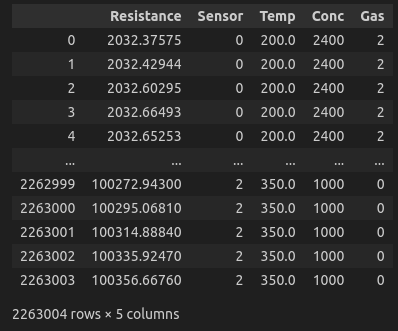
\includegraphics[width=0.5\linewidth]{Thesis Prashant//Images//Results/Screenshot from 2024-04-05 13-49-43.png}
    \caption{Data Head}
    \label{fig:enter-label}
\end{figure}

The resistance column has a range of order 2 to 6; the sensor column consists of three different types of sensors: NiO, CuO, and ZnO. The Temperature column consists of three unique values. 
[2400, 2100, 1800, 1500, 1200,  600,  300,  500,  100,   50,   20,
         10,    5,    2, 2500, 2000, 1000, 2700, 1900, 1700, 1550, 1370,
       1600, 1400,  900,  720,  540,  360,  180,   90,   30] These were the concentration used for sensing in the Conc column.
      The Last column is the target column, which has four types of gases: ethanol, acetone, toluene, and chloroform.

\begin{table}
    \centering
    \caption{Data Overview}
    \begin{tabular}{|c|c|c|c|c|c|}
    \hline
         & \textbf{Resistance} & \textbf{Sensor}  & \textbf{Temp } & \textbf{Conc} & \textbf{Gas}\\
         \hline
        % count & 2.263004e+06 & 2.263004e+06 & 2.263004e+06 & 2.263004e+06 & 2.263004e+06\\
       %  mean  & 2.030207e+05 & 1.146327e+00 & 6.368142e-01 & 1.951900e+01 & 1.429124e+00\\
         %std	&3.152512e+05 & 7.952693e-01 & 9.042883e-01 & 4.789999e+00 & 1.270319e+00\\
         \textbf{min}&8.655768e+02 & 0.000000e+00 & 0.000000e+00 & 0.000000e+00 & 0.000000e+00\\
       %  25\%	&5.910213e+03 & 0.000000e+00 & 0.000000e+00 & 1.600000e+01 & 0.000000e+00\\
        % 50\%	&1.113043e+05 & 1.000000e+00 & 0.000000e+00 & 1.900000e+01 & 1.000000e+00\\
       %  75\%	&2.332103e+05 & 2.000000e+00 & 2.000000e+00 & 2.400000e+01 & 3.000000e+00\\
         \textbf{max}&1.480000e+06 & 2.000000e+00 & 2.000000e+00 & 3.000000e+01 & 3.000000e+00\\
         \hline
    \end{tabular}
    \label{tab:my_label}
\end{table}


\section{Prepossessing Data}
So, our dataset has a total of five columns, the last of which is the target column. Since it is not a numerical attribute and we also want to classify them, it is necessary to hot encode the labels in the target column. so, inside the Gas column (target column) we have
'Gas' encoding: 
         Unique values:  ['Acetone' 'Chloroform' 'Ethanol' 'Toluene']
         Encoded labels:  [0 1 2 3]

and the sensor also has a non-numerical attribute therefore hot encoding is needed\\
'Sensor' encoding: 
         Unique values:  ['CuO' 'NiO' 'ZnO']
         Encoded labels:  [0 1 2] 

Data Processing with one hot encoding for target labels, resistance, and other features was scaled using a min-max scalar in zero to one range. Missing values in the dataset may result in bad model training, so using the mean method to find missing values was also added. Now, the data set has all the numerical values.

To train any model on a dataset, we need to shuffle and split it. Here, $80\%$ of data was used to train the model and $20\%$ of data was kept as a completely new unknown dataset to verify the model externally. That $80\%$ of the data was further used for supervised learning with a train-test split to the same ratio.
Just to see if there are extreme fluctuations in the resistance column, the percentile plot(Fig 2.2) was made. A K-density plot was used to visualize how each gas was distributed.Fig(2.3)

\begin{figure}
    \centering
    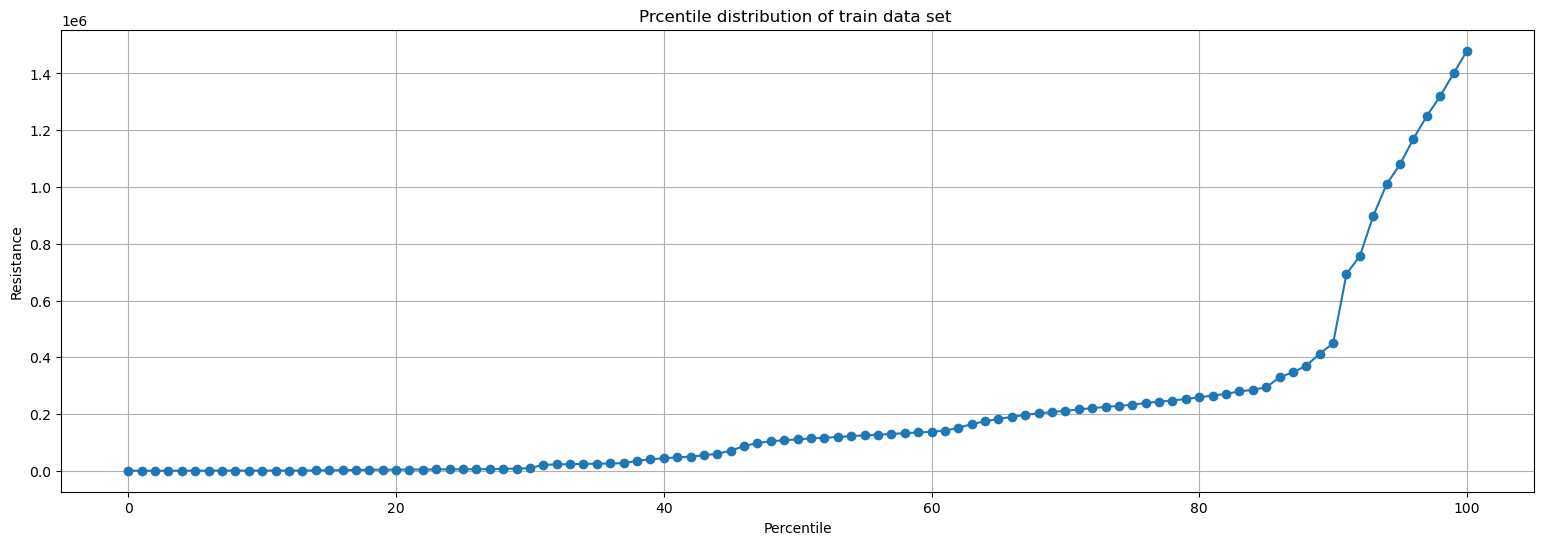
\includegraphics[width=1\linewidth]{Thesis Prashant//Images//Results/percentile plot of data.png}
    \caption{Percentile Plot}
    \label{fig:enter-label}
\end{figure}
\begin{figure}
    \centering
    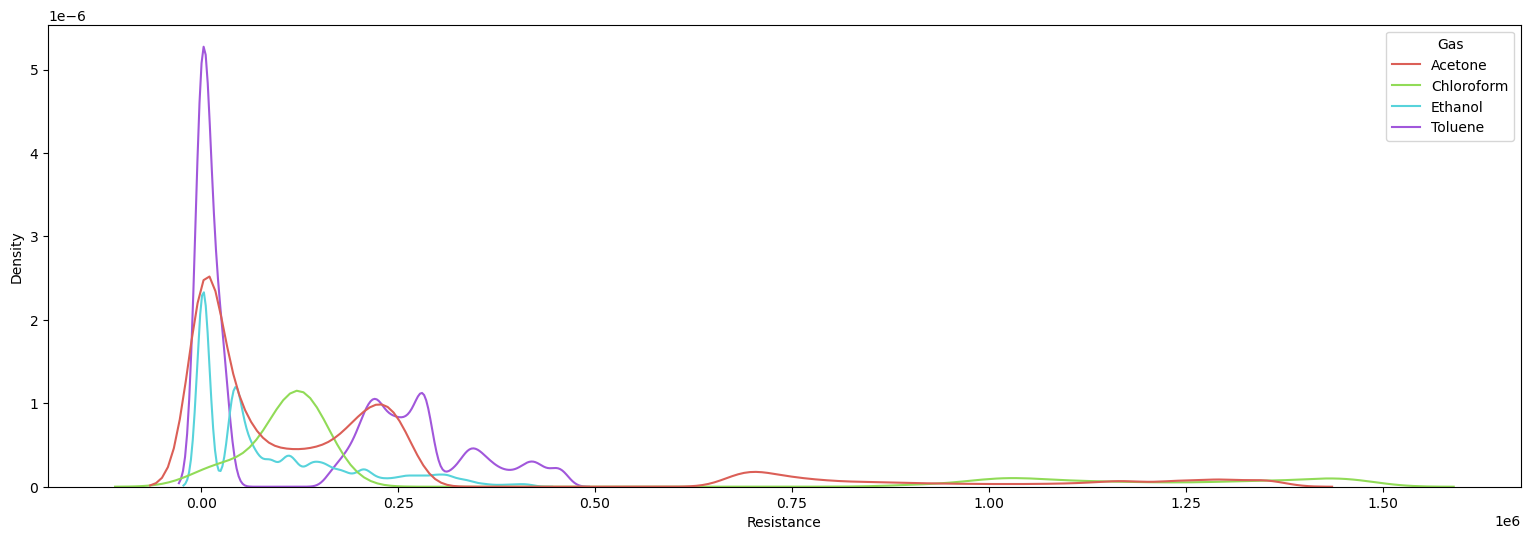
\includegraphics[width=1\linewidth]{Thesis Prashant//Images//Results/KD Plot .png}
    \caption{K-Density Plot of dataset}
    \label{fig:enter-label}
\end{figure}
\chapter{KNN and Decision Tree }
This chapter will analyse the mathematics behind KNN, decision trees, and random forests as multiclass classifiers.
\begin{definition}
\textbf{Shattering} is the ability of a model to classify a set of points perfectly. More generally, the model can create a function that can divide the points into two distinct classes without overlapping. It is different from simple classification because it considers all possible combinations of labels upon those points.
\end{definition}
\begin{definition}\textbf{VC dimension}
    The Vapnik-Chervonenkis dimension, more commonly known as the VC dimension, is a model capacity measurement used in statistics and machine learning. The VC dimension of a model is the size of the largest set of points that that model can shatter.
\end{definition}

\section{KNN} KNN relies on the idea that similar data points tend to have similar labels or values. The KNN algorithm stores the entire training dataset as a reference during the training phase. When making predictions, it calculates the distance between the input data point and all the training examples, using a chosen distance metric such as Euclidean distance.

Next, the algorithm identifies the K nearest neighbours to the input data point based on their distances. In the case of classification, the algorithm assigns the most common class label among the K neighbours as the predicted label for the input data point. For regression, it calculates the average or weighted average of the target values of the K neighbours to predict the value for the input data point.


\subsection{KNN Model}

\begin{algorithm}
\caption{KNN Classification}\label{alg:knn_classification}
\begin{algorithmic}
\REQUIRE Feature matrix $X$ ($n\_samples \times n\_features$), target vector $y$ ($n\_samples$)
\ENSURE Accuracy of the KNN classifier on the test data
\STATE \textbf{Step 1: Split the Data}
    \STATE Split the data into training and testing sets using $train\_test\_split$
\STATE \textbf{Step 2: Import Libraries} import $KNeighborsClassifier$ from scikit-learn and $accuracy\_score$ from scikit-learn.metrics
\STATE \textbf{Step 3: Instantiate the KNN Classifier}
    \STATE Create an instance of $KNeighborsClassifier$ with the desired number of neighbors
\STATE \textbf{Step 4: Train the Classifier}
    \STATE Fit the classifier to the training data
\STATE \textbf{Step 5: Make Predictions}
    \STATE Use the trained classifier to predict the labels of the test data
\STATE \textbf{Step 6: Evaluate the Model}
    \STATE Calculate the accuracy of the model by comparing the predicted labels with the true labels of the test data
\STATE \textbf{Step 7: Output the Results}
    \STATE Print or return the accuracy of the model on the test data
\end{algorithmic}
\end{algorithm}
\begin{itemize}
    \item \textbf{Split data }splitting the data into training and testing sets to evaluate the model's performance is not necessary when using KNN on the same dataset.
    \item \textbf{Import libraries} import the KNeighborsClassifier from scikit-learn.
    \item Instantiate the KNN classifier: Create an instance of the KNeighborsClassifier class. Specify the number of neighbours (n\_neighbors) and other parameters.
    \item \textbf{Train classifier} Fit the classifier to your entire dataset.
    \item \textbf{Make predictions} Use the trained classifier to make predictions on the same dataset.
\end{itemize}
Since predicting on the same dataset trained on, we won't get a true evaluation of the model's performance. So, we used the trained model on a new data set to achieve accuracy.

\subsection{KNN results}
A better model was obtained by KNN with n value 5. For all input features were converted to 0 to 1 as input and target variable hot encoded. The true negative, true positive, false negative, and false positive predictions for the entirely unknown data set of around four lac data points are explained in the confusion matrix.
\begin{figure}
    \centering
    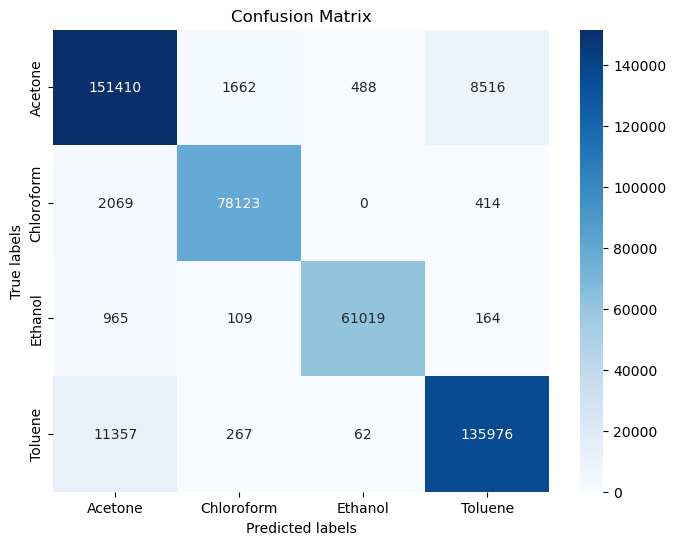
\includegraphics[width=0.8\linewidth]{Thesis Prashant//Images//Results/knn_confusion matrix.png}
    \caption{KNN Confusion Matrix}
    \label{fig:enter-label}
\end{figure}


\section{Decision Tree}

A general framework for growing a decision tree starts with a tree with a single leaf(the root) and assigns this leaf a label according to a majority vote among all labels over the training set. Then, a series of operations are performed. On each iteration, the effect of splitting a single leaf is examined. Then, among all possible splits, we choose the one that maximizes the gain and performs it or chooses not to split the leaf.

A possible Implementation is based on a popular decision tree algorithm known as "ID3" (Iterative Dichotomizer 3), 
the algorithm for the case of binary features, namely, $\xi = {0,1}_{d}$, and therefore all splitting rules are of the form $1_{[x_{i}=1]}$ for some feature $i\in [d]$.

\subsection{Analysis with Decision Tree}
Starting with splitting the data into training and testing sets to evaluate the model's performance 80\% training data and 20\% data for testing was used. Before splitting data, it is shuffled to ensure randomness. The decision tree algorithm from the library was selected and trained. And evaluated using accuracy metrics. After fine-tuning hyperparameters, the algorithm will get better accuracy. After getting the desired accuracy, the model was saved and again used for a completely new data set for cross-validation, and a new confusion matrix was used to visualize the performance of the model.
\subsubsection{hyper-parameters}
Hyperparameters in decision trees are parameters that are set before the learning process begins. They control aspects of the tree's construction and can significantly impact the resulting model's performance and behaviour. 

    \begin{itemize}
        \item \textbf{Criterion} Criterion is the function used to measure the quality of a split. Common options are "Gini" for the Gini impurity and "entropy" for information gain.
        \item \textbf{Max Depth} Max depth controls the maximum depth of the decision tree. It limits the number of nodes in the tree. Setting this parameter helps prevent overfitting.
        \item \textbf{Min Samples Split} Min samples split specifies the minimum number of samples required to split an internal node. The node will not be split if the number of samples at a node is less than this parameter.
        \item \textbf{Min Samples Leaf} Min samples leaf is the minimum number of samples required to be at a leaf node. A split will only be made if it leaves at least this number of samples in each left and right branch.
        \item \textbf{Max Features} Max features determine the maximum number of features to consider when looking for the best split. It can be an integer (considering a fixed number of features) or a fraction (considering a percentage of features).
        \item \textbf{Splitter} Splitter determines the strategy used to choose the split at each node. Options are "best" to choose the best split and "random" to choose the best random split.
        \item \textbf{Min Impurity Decrease} Min impurity decrease is a threshold for the minimum decrease in impurity required for a split to happen. It helps prevent overfitting by requiring a certain amount of improvement in purity.
        \item \textbf{Class Weight} lass weight is used to handle class imbalance. It assigns weights to different classes to balance their representation in the tree.
        \item \textbf{Presort} Presort specifies whether to presort the data to speed up the finding of best splits during training. It is generally not recommended for large datasets.
    \end{itemize}

\subsection{Decision Tree Results}
A model was obtained by a Decision tree for all attributes that were converted to 0 to 1 as input and target variable hot encoded. The true negative, true positive, false negative, and false positive predictions for the entirely unknown data set of around four lac data points are explained in the confusion matrix).
\begin{figure}
    \centering
    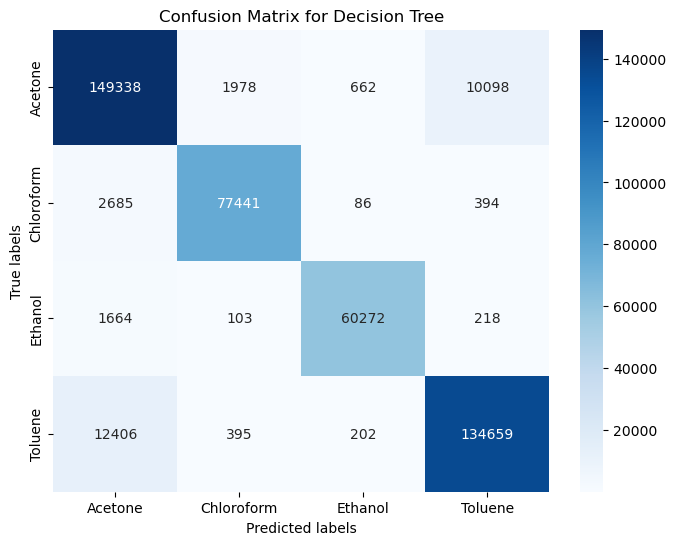
\includegraphics[width=0.8\linewidth]{Thesis Prashant//Images//Results/Confusion Decision.png}
    \caption{Confusion Matrix Decision Tree}
    \label{fig:enter-label}
\end{figure}

\subsection{Random Forest}
The Class of Decision Tree of arbitrary size has infinite VC dimension. So, a restriction on the size of the decision tree is needed. The danger of overfitting can be reduced by constructing an ensemble of trees. the method of $random forests$ was introduced by Breiman(2001). A random forest is a classifier consisting of a collection of a collection of decision trees, where each tree is constructed by applying an algorithm A on the training set S and an additional random vector, $\theta$, where, $\theta$ is sampled independent and identically distributed from distribution. A majority vote over the individual trees' predictions obtains the random forest's prediction.

\subsection{Random Forest Results}
A better model was obtained by Random Forest for all attributes that were converted to 0 to 1 as input and target variable hot encoded. The true negative, true positive, false negative, and false positive predictions for the entirely unknown data set of around four lac data points are explained in the confusion matrix.
\begin{figure}
    \centering
    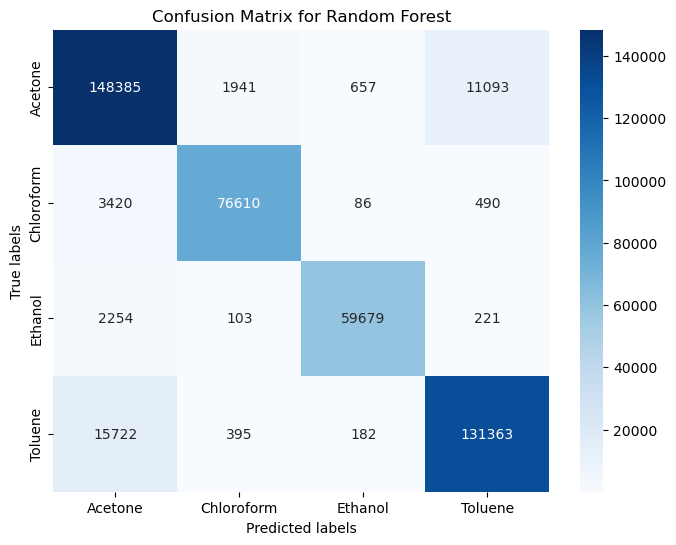
\includegraphics[width=0.8\linewidth]{Thesis Prashant//Images//Results/confusion_random_forest.png}
    \caption{Confusion Matrix Random Forest}
    \label{fig:enter-label}
\end{figure}
% Remember to input this to the presentative tex file before compiling.
\chapter{Neural Networks Based Classifiers}

Classification problems for a complex and large dataset with unpredictable results using linear methods can be calculated using neural networks, which can be trained to adjust with the result requirements. Also, once we train the network, it can be used on any similar dataset efficiently and with higher accuracy. Neural networks are just a set of functions that change themselves to learn and fit into a model. 

\section{How Neural Networks Works}
Neural networks are computational models inspired by the structure and function of the human brain. It consists of interconnected nodes in this case neurons, organized into layers. Each neuron receives input signals, processes them using an activation function, and produces an output signal. Layers are typically organized into an input layer, one or more hidden layers, and an output layer. The input layer receives raw data, while the output layer produces the model's predictions or classifications. There are hidden layers between the input and output layers, where the network learns to predict the result from the input data. Each connection between neurons is associated with weights, and each neuron also has a bias term. During training, the network adjusts these weights and biases using an optimization algorithm to minimize the loss function, which measures the difference between the predicted output and the true labels.\\
A neural network is trained by giving it labelled training data and modifying its weights and biases to reduce the difference between the labels it predicts and the actual labels. This is done through an iterative process of forward propagation, loss calculation, and backpropagation. In forward propagation, input data is passed through the network, layer by layer. At each layer, the input is transformed by the weights and biases of the neurons and then passed through the activation function to produce an output, and this Output becomes the Input of the next layer. This process continues until the output layer is reached, producing the model's prediction.
After getting the Output at the end of the last layer, the loss function is calculated by comparing the predicted output to the true labels or target values. Common loss functions are mean squared error for regression tasks and cross-entropy loss for classification tasks. The network then adjusts its weights and biases through backpropagation, by computing the gradient of the loss function with respect to each weight and bias in the network and updating them accordingly. This process continues for a predefined number of iterations (epochs) or until the model's performance on a separate validation dataset reaches a satisfactory level of result.

\section{Architecture of Neural Network}
A neural network consists of many neurons called nodes. Their amount could be from a couple of dozen to even millions, and they are arranged in layers. All the nodes can be classified into input, hidden, and output nodes, which connect the layers on either side. 

% picture workflow of neural network

The Input layer consists of input nodes responsible for receiving numerical data from outside of the dataset that the neural network attempts to learn about. The connection between one node from the input layer and one from the hidden layer is represented by a number called weight, which is denoted as $W_{i}$. The weight can be positive or negative, corresponding to how brain cells excite or suppress others. If a node has a higher corresponding weight, then it has more influence on the output. Initially, the weights are assigned randomly and are adjusted later in the training process.

In neural networks, information can flow through a neural network in two ways. The simplest type of Neural network is Feedforward Neural Network. In Feedforward Neural Network, the data value goes only in one direction, from the input nodes to hidden nodes, and then finally to the output nodes.
%Exapmle Picture of Feedforward Neural Networks

The Input layer Collects the numerical variables from the Dataset and carries them to the next stage, no computation happens here. Then, the data values are at the first hidden layer, which has an activation function. The activation functions perform computations and transfer the new values to the next hidden layer or output layer. A feedforward network will only have a single Input layer, and it can also have zero or multiple hidden layers.
The output layer contains all output nodes, which our results computed from prior hidden layers can be considered. One type of neural network, known as a recurrent neural network, has a loop or cycle connecting all the nodes inside it. The recurrent attribute allows it to exhibit temporal dynamic behaviours.


\subsection{Forward Neural Networks}
Neural networks refer to the complex links among neurons; communication links can join many neurons to carry out complex computations. The structure of a neural network can be described as a graph whose nodes are the neurons, and each edge in the graph links the output of one neuron to the input of another neuron. For the feed-forward network structure, the graph does not contain any loop.
A feed-forward neural network can be described by a directed acyclic graph, G = (V, E), and a weight function over the edges, $w: E\xrightarrow{}R$. Nodes of the graph can be considered as neurons. Each single neuron is moulded as a simple scalar function, $\sigma: R\xrightarrow[]{}R$.
$\sigma$ can be a 

sign function, $$\sigma(a) = sign(a)$$

threshold function, $$\sigma(a) = 1_{[a>0]}$$

the sigmoid function, $$\sigma(a) = \frac{1}{1+\exp{-a}}$$

The sigmoid function is a smooth approximation to the threshold function. $\sigma$ is called the "activation function" of the neuron.
Each edge in the graph links some neuron's output to another neuron's input. The input of a neuron is calculated by taking a weighted sum of the outputs of all the neurons connected to it, weighting can be tweaked by $w$.
Assume that the network is organized in \textit{layers}, that is, the set of nodes can be decomposed into a union of nonempty disjoint subsets, $V=\bigcup_{t=0}^{T}V_{t}$ (disjoint union), such that every edge in E connects some node in $V_{t-1}$ to some node in $V_{t}$, for some $t\in [T]$.

The bottom layer, $V_{0}$ is called the input layer. It contains n+1 neurons, where n is the dimension of the input space. For every $i\in[n]$, the output of neuron $i$ in $V_{0}$ is simply $x_{i}$.
The last neuron in $V_{0}$ is the "constant" neuron, which always outputs 1.

let's denote $v_{t,i}$ the $i$th neuron of $t$th layer
and $o_{t,i}(X)$ the output of $v_{t,i}$ when the network is fed with the input vector $x$.
Therefore, for $i\in[n]$ we have $o_{0,i}(x) = x_{i}$ and for $i = n+1$ we have$o_{0,i}(x)=1$.
Let's calculate in a layer-by-layer manner. Suppose we have already calculated the outputs of neurons at layer $t$.

Then, we can find the outputs of the neurons at layer $t+1$ by fixing some $v_{t+1,j}\in V_{t+1}$.
Let $a_{t+1,j}(x)$ denote the input to $v_{t+1,j}$ when the network is fed with the input vector $x$.

Then, $$a_{t+1,j}(x) = \sum_{r:(v_{t,r},v_{t+1,j})\in E}w((v_{t,r},v_{t+1,j}))o_{t,r}(x),$$ and $$o_{t+1,j}(x) = \sigma( a_{t+1,j}(x)) .$$

The input to $v_{t+1,j}$ is a weighted sum of the outputs of the neurons in $V_{t}$ that are connected to $v_{t+1,j}$, where weighting is according to $w$, and the output of $v_{t+1,j}$ is simply the application of the activation function $\sigma$ on its input.

Layers $V_{1},\cdots,V_{T-1}$ are often called \textit{hidden layers}. The top layer $V_{T}$ is called the Output Layer.
In Simple prediction problems, the output layer contains a single neuron whose output is the output of the network.

Let's Refer to $T$ as the number of layers in the network(excluding $V_{0}$) or the "depth" of the network. The size of the network $\mod{V}$. the "width" of the network is $max_{t}\mod{V_{t}}$. See Figure Below. A layered feedforward neural network of depth 2, size 10, and width 5 is given for better understanding.

Note that a neuron in the hidden layer has no incoming edges. this neuron will output the constant $\sigma(0).$

\subsection{Activation Function}
An activation function takes the dot-product mentioned before as an input and performs a certain computation on it.
A notable property of activation functions is that they should
be differentiable because this property is needed to train the neural network using backpropagation optimization.

\subsubsection{Sigmoid or Logistic}It takes a real-valued input and returns a output in range[0,1]
$$\delta(x)=\frac{1}{1+e^{-1}}$$ 
\textbf{sigmoid activation function picture}\\
In Fig, this is an S-shaped curve, and the values going through the Sigmoid function will be squeezed in the range of [0, 1]. Since the probability of anything exists only between the range of 0 and 1, Sigmoid is a compatible transfer function for probability. Although the Sigmoid function is easy to understand and ready to use, it is not used frequently because it has a vanishing gradient problem. This problem is that, in some cases, the gradient gets so close to zero that it does not effectively apply change to the weight. In the worst case, this may completely stop the neural network from further
training. Second, the output of this function is not zero-centered, which makes the gradient updates go far in different directions. Besides, the fact that output is in the narrow range [0, 1] makes optimization harder. In order to compensate for the shortcomings, the $tanh()$ function is an alternative option because it is a stretched version of the Sigmoid function, in which its output is zero-centred.
\subsubsection{$tanh$ or hyperbolic tangent:}
it takes real-valued input and produces the results in the range[-1,1]:
$$tanh(x) = \frac{\sinh{x}}{\cosh{x}}=\frac{e^{x}-e^{-x}}{e^{x}+e^{-x}}$$
The advantage is that the negative input values will be mapped strongly negative and zeros will be mapped near zero through this function. Therefore, this function is used when classification is needed to be performed between two classes. In practice, this function is preferred over the sigmoid function, but the gradient vanishing problem still exists. so the ReLU function is used
\subsubsection{ReLU} Rectified Linear Unit function takes a real-valued input and replaces the negative values with zero
$$R(x) = max(0,x)$$
The ReLU() activation function is trending now in the field of neural networks. It is used in almost all convolutional neural networks or deep learning because it is a relatively simple and efficient function that avoids and rectifies the gradient vanishing problem. The problem with this activation function is that all the negative values become zeros after this activation, which in turn affects the results by not taking negative values into account. A different activation function can be used when we know what characteristics of results we expect to see. Among these three activation functions, we usually start our training process using ReLU() because it works as a general approximator for most data sets.

\subsection{ Multi-Layer Perceptron} there are two types of feed-forward neural networks:
\begin{itemize}
    \item Single layer Perceptron: the simplest feed-forward neural network with no hidden layers.
    \item Multi-layer Perceptron: it has more than one layer, which is useful for practical application
\end{itemize}

Multi-layer perceptron can learn not only linear functions but also non-linear functions. The feed-forward neural network in Figure is an example of the multi-layer Perceptron. For a data set containing features and results, the multi-layer Perceptron will learn the relationship between features and results from the given data set and predict the result for
a new data point. Generally, in the input layer, we send n numerical inputs through n nodes:$$ x = x_{1},x_{2},\cdots,x_{n} |x\in R^{n}$$
then randomly assign weights for them in the first place: $$w = w_{1},w_{2},\cdots,w_{n}$$ the values for weights will be adjusted later in the training process for more accurate approximations.\\
In the hidden layer, all the inputs by taking the dot product of x and w, and is known as the pre-state P
$$P = w_{1}\cdot x_{1}+w_{2}\cdot x_{2}+\cdots+w_{n}\cdot x_{n}+b$$
$$ P = \sum^{n}_{i=1}(x_{i}w_{i}) + b$$

\begin{figure}
    \centering
    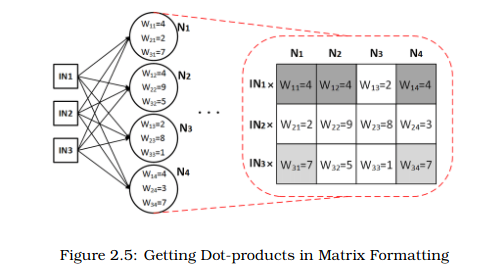
\includegraphics[width=0.6\linewidth]{Thesis Prashant//Images//media/Screenshot from 2024-04-23 00-29-37.png}
    \caption{Dot-products in Matrix Formatting}
    \label{fig:enter-label}
\end{figure}


Let's use vectors to represent them so that it can be treated as a matrix format. In Fig, the input layer has 3 nodes, and the following hidden layer has 4 nodes. Let's create a matrix of 3 rows and 4 columns and insert the values of each weight in the matrix as done above. This matrix would be called $W_{1}$. A 1 × 4 pre-state matrix can be obtained by matrix multiplication. In the hidden layer, four pre-states $N_{i}$, each store the dot-product of corresponding inputs and weights. These four pre-state values are ready to go through a certain activation function σ(). This is called the state S inside this hidden neuron.$$ S = \sigma(W_{i}IN_{i} +b)$$
There could be more hidden layers following the first hidden layer, and the state(s) S, which stores the transformed values, will be the input value(s) for the next layer. The matrix contains all the state values that will encounter the next weight matrix and produce new dot-products, and at that time, all the state values become the pre-state values of the next stage. The initial input values will go through every hidden layer in the neural net, repeat the same procedure mentioned above, and finally arrive at the output layer. The output values we receive are the ultimate state values in the very last hidden layer. This procedure explains how we set up our neural net.

%Now the question is, how do we determine the weights? How do we adjust the weights so that neural networks make more accurate predictions?

\subsection{Model Building}
A neural network learns from patterns of data and tries to make predictions as accurately as possible. Assume that we already have a set of $p$ data pairs containing the variables and the results, $(x^{(1)},t^{(1)}),(x^{(2)},t^{(2)}),\cdots, (x^{(p)},t^{(p)}),$ where $x^{(i)}$ is input value and $t^{(i)}$ is the target value for i=1, 2, 3, ..., p. We would like to build a neural net $F$ so that ideally, $$F(x^{(i)}) = t^{(i)}$$
typically for $\epsilon_{i}$. Let $y^{(i)}$ denote the output of the  neural network so that 
$$y^{(i)} =F(x^{(i)})  \text{ and } t^{(i)} = y^{(i)} + \Vec{\epsilon_{i}}$$
here $y^{(i)}$ depends on parameters, which are weights and biases, then it turns out as an optimization problem. so we need to set a neural network F that minimizes the error function, which is denoted by E
$$ E = \frac{1}{N} \sum_{i=1}^{p}||t^{(i)}-y^{(i)}||^{2}$$
where N is the number of training patterns. If it is a two-way classification problem, then N = 2. From this equation, E is a function of the parameters in F, and we need to determine the values of weights that minimize the error by differentiating E. Let's focus on only one term of the sum, then
$$||t-y||^{2} = (t_{1}-y_{1})^{2}+(t_{2}-y_{2})^{2}+\cdots+(t_{p}-y_{p})^{2}$$
because it is already known that the input and output values are fixed, and the only parameter here is the weight. We can differentiate both sides and get
$$\frac{\delta}{\delta W}(||t-y||^{2}) = -2(t-y)\cdot\frac{\delta y}{\delta W}$$
from neural network the output is $y^{(i)} = W_{ij}x^{(i)}+b$ 
Clearly, the output depends on the weight and if we differentiate both sides with respect to $W_{ij}$ using the chain rule, we get$$\frac{\delta}{\delta W_{ij}}(||t-y||^{2}) = -2(t_{i}-y_{i})x_{j}$$
here$x_{j}$ is the $i^{th}$ coordinate position.
This derivative gives us the direction to the maximum, so in order to obtain the minimum point, we follow the opposite direction of this gradient. Additionally, it is desired to see this derivative as close to 0 as possible in order to obtain the minimum error. 
%This algorithm follows the Widrow-Hoff Rule(see Appendix).
After figuring out which direction to go, we still need to know how far we go. We do not want it to move too slowly because we would like to finish this training part in an efficient manner. On the other hand, we do not want it to move a step too far; we may face the problem of not converging. Learning rate α is an important hyperparameter in
gradient descent because it determines how far each step should go. Unfortunately, we cannot analytically calculate a learning rate for a certain data set; we can know it only through trial and error. Typical values for a neural network with standardized inputs (or inputs mapped to the (0,1) interval) are less than 1 and greater than $10^{-6}$.

%-------------------------------------------------------------------------Back Propogation 
\subsection{Back Propagation}
Backward propagation or backpropagation is the process of propagating the error or loss back to the neural network and updating the weights of each neuron subsequently by adjusting the weight and bias parameters.

Back-propagation plays an important role in the Neural Network. It performs several mathematical operations to learn the patterns between the input and the target variable.
The main goal of the neural network is to get the minimum error(loss). We can achieve a minimum error between an actual target value and a predicted target value if we get the correct value of the weight and bias parameters.
The error keeps changing with respect to the parameters. This rate of change in error is to be found by calculating the partial derivation of the loss function with respect to each parameter.

By performing derivation, one can determine how sensitive is the loss function to each weight & bias parameter. This method is also known as the Gradient Descent optimization method.

Let's start with a simple 1-1-1 neural network, which contains an input $x$, two stages of weights, $w_{1}$, $w_{2}$, two stages of biases, $b_{1}$, $b_{2}$, an activation function $\sigma()$ and an output $y$.
$$y = w_{2}\sigma(w_{1}x+b)+b_{2}$$
Given a target $t$, the error of this neural net is $$ E(w_{1},w_{2},b_{1},b_{2}) =\frac{1}{2}(t-y)^{2}$$
$$ = \frac{1}{2}(t- (w_{2}\sigma(w_{1}x+b_{1})+b_{2}))^{2}$$ 
to minimize the error, we need to move in the opposite direction of the gradient. Through the training process, we would like to update weights/biases in order to achieve a better error. Suppose we let $u$ denote a generic parameter (either a weight or a bias). Using the gradient descent, $u$ is updated by:
$$u_{new} = u_{old}-\alpha\frac{\delta E}{\delta u} = u_{old}+ \alpha\Delta u$$
Where $\alpha$ is called the learning rate, and the change in $u$ is computed via the chain rule on the error. Notice that we incorporated the negative sign into ∆u, because the derivative of the $(t − y)$ term will always be negative $t − y$. In particular,
$$\Delta u = - \frac{\delta E}{\delta y}\cdot\frac{\delta y}{\delta u}$$
$$ = -(t-y)\cdot - \frac{\delta y}{\delta u}$$
$$ = (t-y)\frac{\delta y}{\delta u}$$
Recall the pre-state P (pre-state) and state S mentioned in the prior section,
$$ P = w_{1}x + b_{1} \space S=\sigma(P)$$
Now, Let us compute these partial derivatives for all different parameters:
for $y= w_{2}S+b_{2}$ ,
$$ \frac{\delta y}{\delta w_{2}} = S \text{  , } \frac{\delta y}{\delta b_{2}} = 1$$
$$ \Delta w_{2} = (t-y)S \text{   , }\Delta b_{2} = (t-y)$$,

for $y= w_{2}\sigma(P)+ b_{2}$ ,
$$ \frac{\delta y}{\delta w_{1}} = w_{2}\sigma'(P)\cdot x \text{  , } \frac{\delta y}{\delta b_{1}} = w_{2}\sigma'(P)$$
$$ \Delta w_{1} = (t-y)w_{2}\sigma'(P) \text{   , }\Delta b_{1} = (t-y)w_{2}\sigma'(P)$$,
From the example of a 1-1-1 neural net, we can generalize this to a three-layer neural network in the form of n−k−m with the activation function $\sigma$. Although we could define a different σ for every neuron, we typically use the same activation function for all the neurons in a single layer. Once that is done, we have to find matrices $W_{1}, W_{2}$ (and more, if we use more layers) and the bias vectors $b_{1}, b_{2}$.

Ideally,  much more data is needed in order to get good estimates. The key idea is that once we have the derivative of the sum of squares error with respect to the weights, we can adjust the weights accordingly through the training process.
%In practice, the algorithm for reducing the error function is already stored in the neural network, so we only need to set up a neural network using software (e.g. Matlab), and we can see the training process happens automatically.


\section{stochastic gradient descent}
Stochastic Gradient Descent Method \cite{shalevshwartz2014understanding} 


\subsection{Gradient Descent}
The gradient of a differentiable function $f:R^{d} \xrightarrow{}{}R$ at $w$, denoted $\nabla f ($W$)$, is the vector of partial derivatives of $f$.

$$\nabla f(w) = \left(\frac{\partial f(w)}{\partial w[1]},\cdots,\frac{\partial f(w)}{\partial w[1]}\right)$$.

A gradient is an iterative algorithm. let's start with initial value of $w$, $w^{1} = 0$.
then, at each iteration, take a step in the direction of the negative of the gradient at the current point. 
that will be the updated step 
$$w^{t+1} = w^{t}-\eta\nabla f(w^{t})$$,
$\eta>0$ will be discussed later. Since the gradient points in the direction of the direction of the greatest rate of increase of around $w^{t}$, the algorithm needs to make a small step in the opposite direction, thus reducing the value of the function. After $T$ iteration the algorithm outputs the averaged vector,
$$\bar{w} = \frac{1}{T}\sum_{t=1}^{T} w^{t}$$
The output could also be the last vector, $w^{T}$, or the best-performing vector. However, taking the average would be better, especially when generalising gradient descent to non-differentiable functions and the stochastic case.


\section{Neural Network Classification Model}
These are the Steps followed here to train the neural model for better accuracy


\begin{algorithm}
\caption{Neural Network Training and Evaluation}\label{alg:neural_network}
\begin{algorithmic}
\STATE \textbf{Input}: $X$, $y$ (features and labels), $X_{\text{train}}$, $X_{\text{test}}$, $y_{\text{train}}$, $y_{\text{test}}$ (training and testing splits)
\STATE Initialize neural network model $model$
\STATE Add layers to $model$: 64-neuron dense layer with ReLU activation, 64-neuron dense layer with ReLU activation, 4-neuron dense layer with softmax activation function
\STATE Compile $model$ with Adam optimizer and sparse categorical crossentropy loss
\STATE Train $model$ on $X_{\text{train}}$ and $y_{\text{train}}$ for 50 epochs with batch size 32 and 10\% validation split
\STATE Evaluate $model$ on $X_{\text{test}}$ and $y_{\text{test}}$ to calculate loss and accuracy
\end{algorithmic}
\end{algorithm}

\begin{itemize}
    \item \textbf{Data Preparation} Splitting dataset into features (X) and target (y), then further splitting them into training and testing sets using train\_test\_split.
    \item \textbf{Model Definition}Defining a neural network model using the Sequential API. This model consists of three Dense layers. The first two layers have 64 neurons, each with ReLU activation function, and the final layer has 4 neurons with softmax activation function, suitable for multiclass classification.
    \item \textbf{Model Compilation}Compiling the model using the Adam optimizer and sparse categorical crossentropy as the loss function and specifying accuracy as the metric to monitor during training.
    \item \textbf{Model Training}Training the model on the training data (\textit{X\_train, y\_train}) for 50 epochs with a batch size of 32. Additionally, using 10\% of the training data as a validation set during training.
    \item \textbf{Model Evaluation}Finally, evaluate the trained model on the test data (X\_test, y\_test) and obtain the loss and accuracy scores.
\end{itemize}



\section{Neural Networks Results}
For all the features converted to 0 to 1 as input and target variable hot encoded, different neural network parameters were tweaked to get a better model. See Table 4.1. it shows 32 batch size and 50 epochs will be enough with $10\%$ validation split. The confusion matrix explains about the true negative, true positive, false negative and false positive prediction for the completely unknown data set with around four lac data points.

\begin{table}
    \centering
    \caption{Training Neural Network Model}
    \begin{tabular}{|c|c|c|c|C|c|}
    \hline
    \textbf{epoch} & \textbf{Batch size} & time & validation split & Loss & Accuracy \\
    \hline
    500 & 256 &7m& 0.1 &  0.139866 & 0.9316594\\
    500 & 64 &140m& 0.1 &  0.12724 & 0.937797\\
    100 & 128 &14m& 0.1 &  0.13216 & 0.9351769\\
    100 & 64 &28m& 0.1 &  0.131524 & 0.935428\\
    100 & 16 &110m& 0.1 &  0.181495 & 0.9097726\\
    50 & 128 &7m& 0.1 &  0.15372 & 0.922419\\
    50 & 32 &28m& 0.1 &  0.1405129 & 0.933256\\
    50 & 32 &27m& 0.2 &  0.1404415 & 0.932207\\
    50 & 32 &23m& 0.1 &  0.134115 & 0.93225824\\
    \hline
    \end{tabular}
    \label{tab: Training_Neural_Network }
\end{table}

\begin{figure}
    \centering
    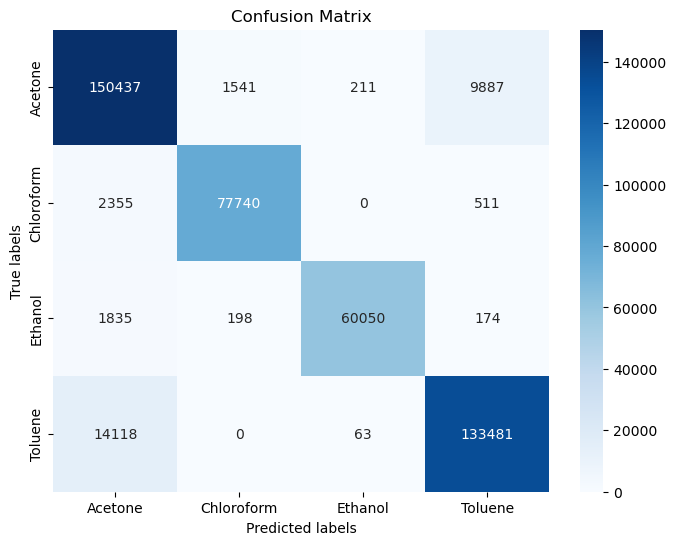
\includegraphics[width=0.8\linewidth]{Thesis Prashant//Images//Results/confusion_matrix_new_dataset.png}
    \caption{Confusion Matrix for trained neural networks on New Data set}
    \label{fig:enter-label}
\end{figure}

\chapter{Multi-Sensor Array}
The ML analysis was recorded for three sensors, and each sensor was maintained at a sufficiently high temperature in order to achieve a decent sensor response. However, each sensor material (oxides in this case) may have its optimum temperature at which the response would be highest, and this optimum response temperature need not be the same for all materials used. Therefore, compared to the previous method of measurement, where all the sensors are kept at the same temperature (See Appendix C), a new setup was designed and built wherein a sizable number of sensor arrays (6 nodes) may be accommodated. The temperature of each can be controlled individually such that each of them is at its optimal temperature. Besides, one can also program the heater power supply to the desired waveform to tune the sensor response dynamically, and that could be used as an effective control feature of ML data.
\begin{figure}
    \centering
    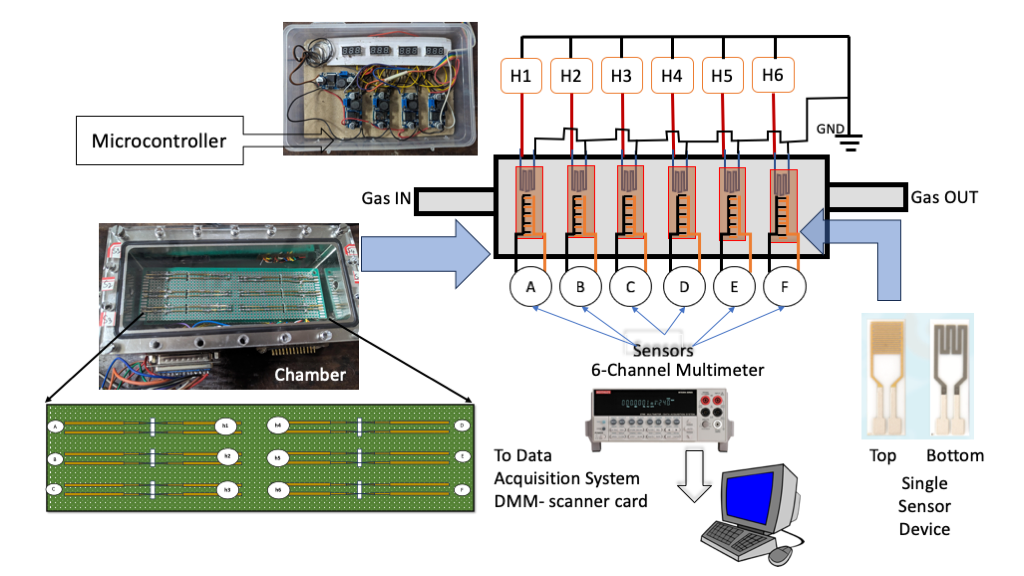
\includegraphics[width=1\linewidth]{Thesis Prashant//Images//Figures/Picture_presentation.png}
    \caption{Schematics of six sensor arrays with individual heater control using microcontroller and the sensor output leads (Interdigitated gold electrodes) to simultaneously measure sensor response of 6 nodes. The typical single-sensor device is shown with top electrodes and a bottom heater.}
    \label{setupl}
\end{figure}

The new setup built is shown in Fig 5.1. It can accommodate up to six sensors simultaneously, as seen in the figure. A metallic chamber containing two layers where one PCB Snaps on the other and holds the top PCB consist of six-hole slits where alumina samples with deposited heaters can be slid. On each side horizontal to the PCB slit, two pogo pins were used to make contact with the alumina sample electrode or heater, exploiting the spring-loaded mechanism of pogo pins. Similarly, six samples may be fitted in a single top PCB. The other side of the PCB contains 2.54 mm pins, which simply snap onto the bottom PCB. The Bottom PCB is fixed inside the chamber with all the wiring and connection to a 25-pin connector side to the wall of the chamber, as shown in the figure. A transparent lid is used to enclose the chamber from the top. The metal chamber has inlet and outlet pipes to achieve gas flow. 

The whole assembly consist of six sensors and six heaters. The Pt deposition on the alumina substrate on one side acts as a heater with $6 \Omega$ resistance, ensuring precise and local heating. On the other hand, the opposite side of the alumina provides the surface for the sensor substrate. A multi-channel voltage supply was also constructed using a parallel six-buck converter to drive the heater at a constant temperature individually. The main voltage source for all the buck converters was a 24 V-5 A SMPS (Switch Mode Power Supply). The buck converter gives the freedom to adjust the constant voltage individually by changing its potentiometer. Hence temperature of the each sensor can be controlled, for better utilization a micro controller can be used to set the temperature simultaneously for each sensor by changing the voltage on buck converter. The heater can go up to $450^\circ C$ at 12 V. So the Bottom PCB inside the chamber provides the interface to connect all the sensors to the voltage supply source and multi-meter to measure the resistance. 

\begin{figure}
    \centering
    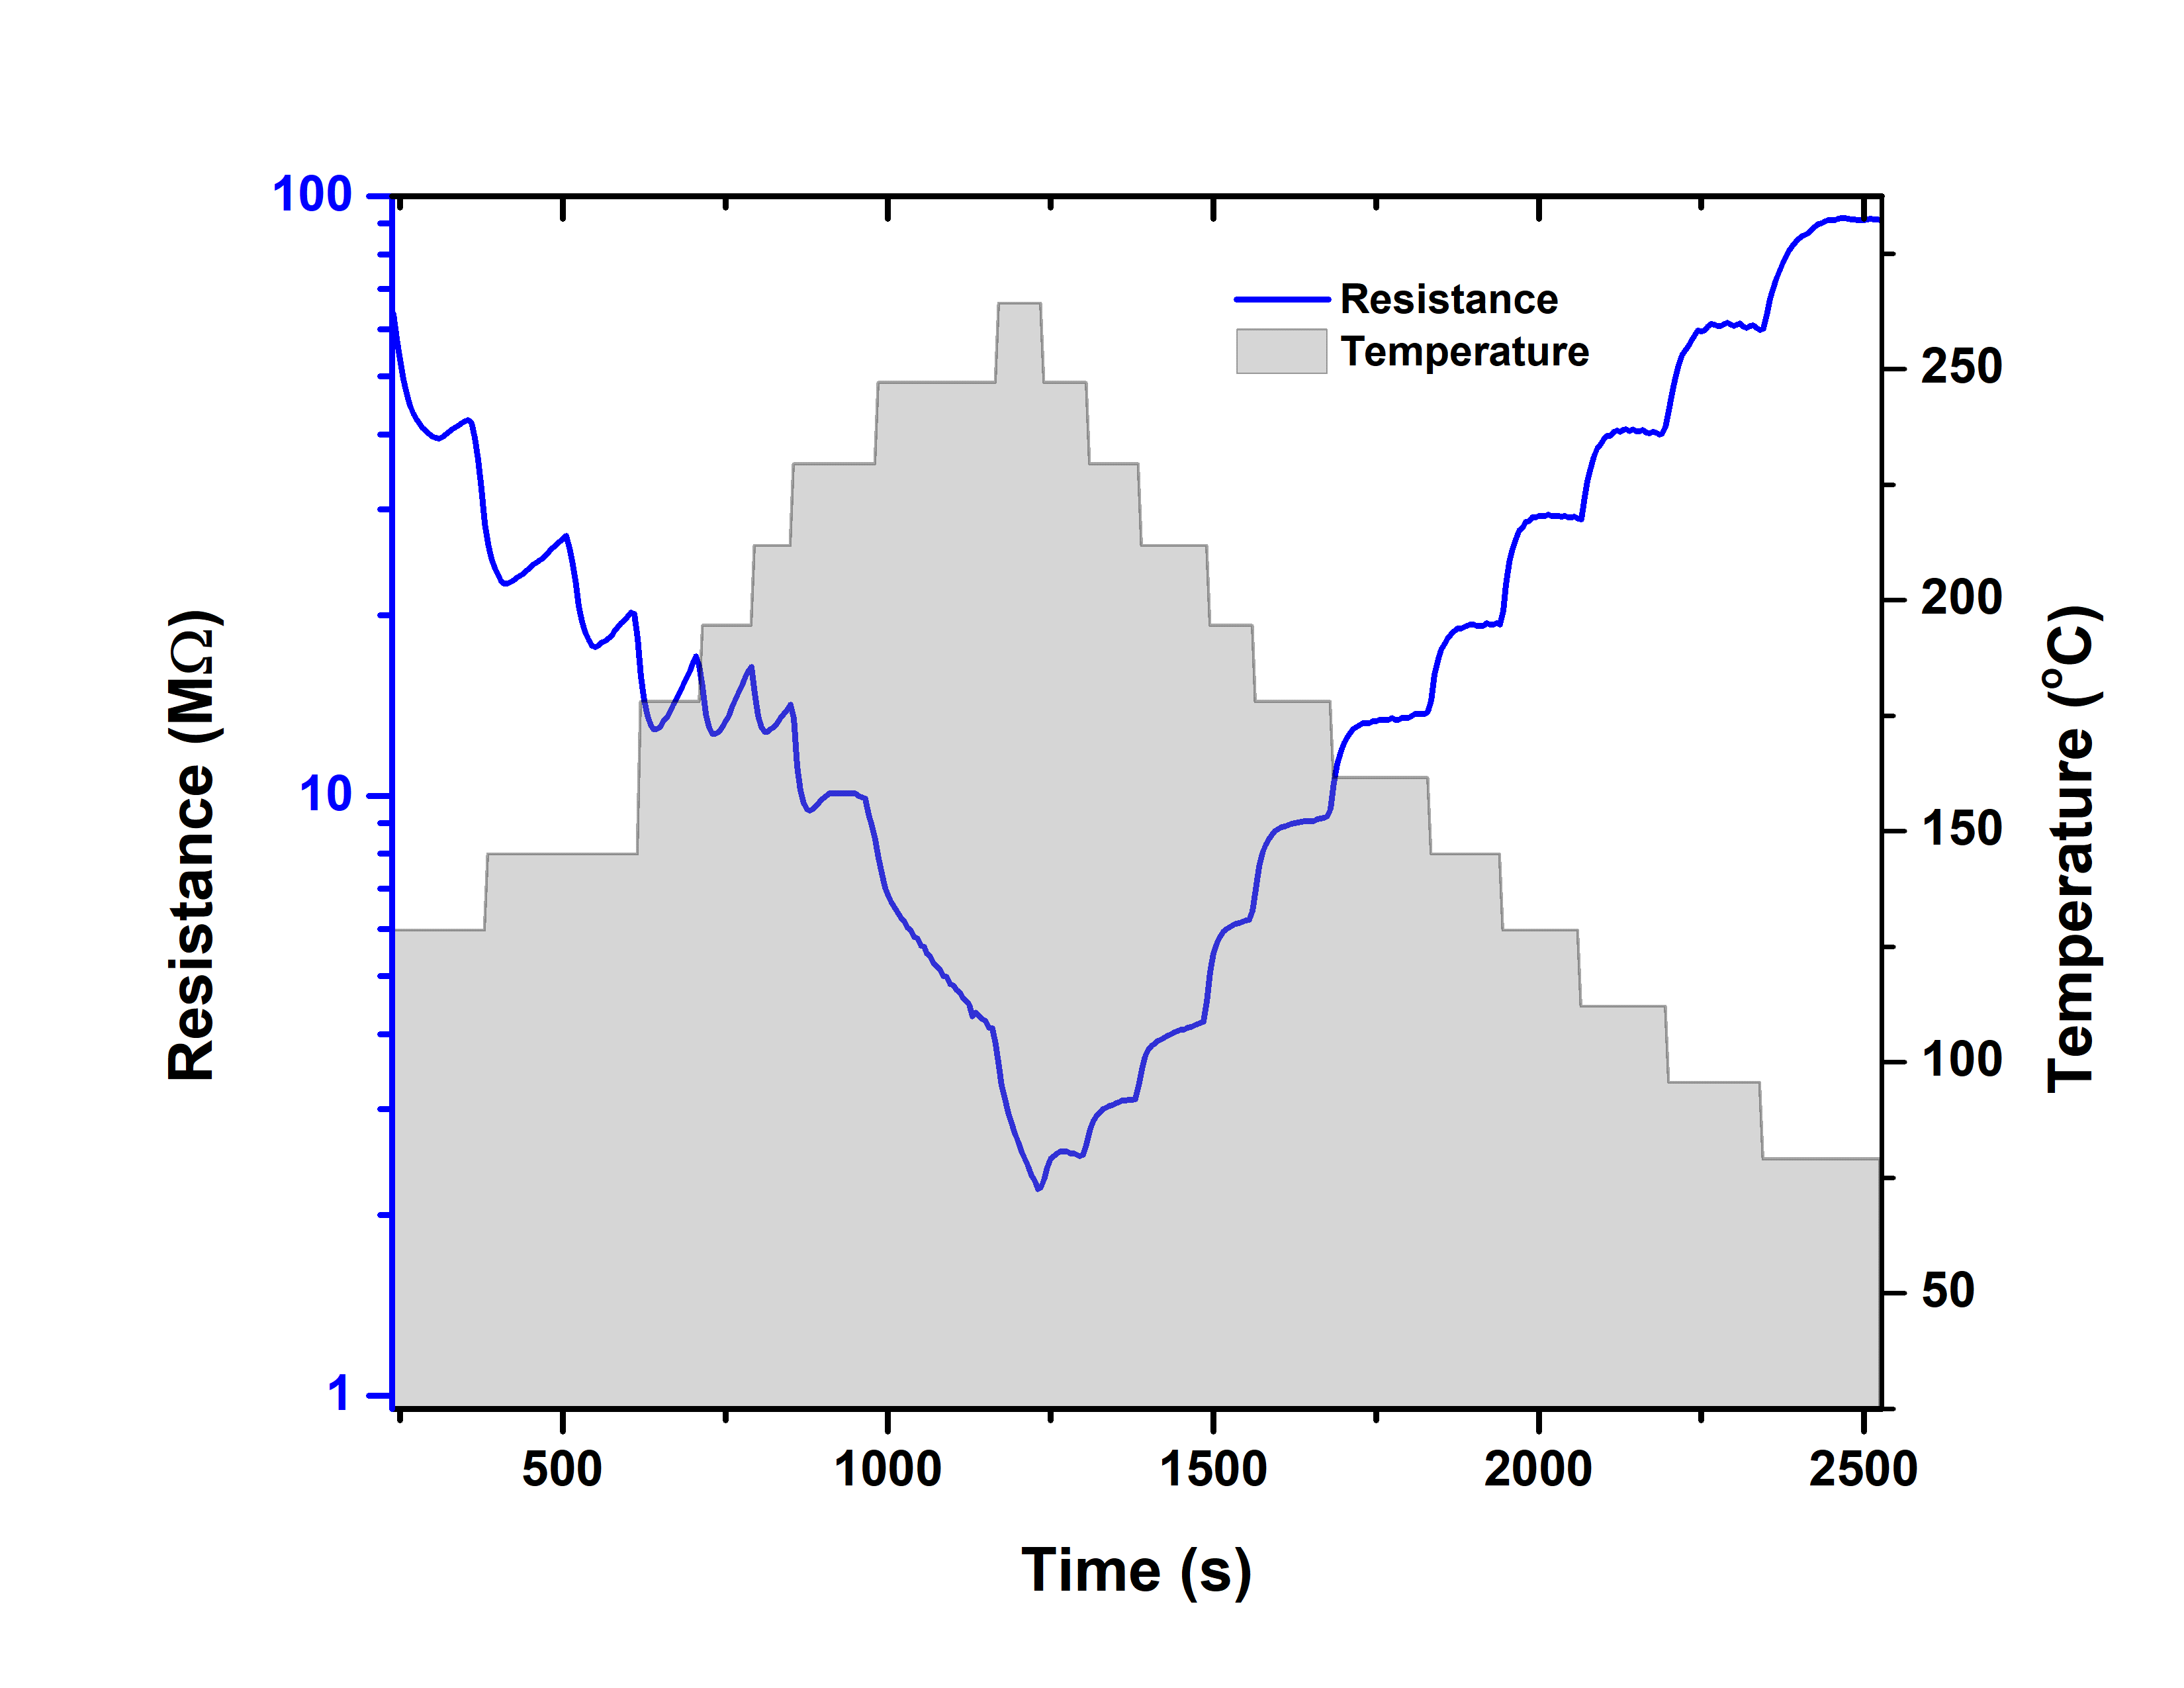
\includegraphics[width=1\linewidth]{Thesis Prashant//Images//Figures/Graph10.png}
    \caption{The data recorded with the assembly described in Fig 5.1 for a single sensor using a controller made. (measurement courtesy Ms. Niharika)}
    \label{fig:setup}
\end{figure}



% Remember to input this to the presentative tex file before compiling.
\chapter{Conclusion}
\begin{itemize}
    \item The aim of the project involves multi-sensor data analysis and designing a set-up to characterise devices for the identification of gases. 
    \item The data collected with 3 sensor arrays was analysed using machine learning techniques.
    \item The main method for analysis relied on the dimensional reduction method to visualise data and ML methods for the classification of the data.
    \item The comparison of the classification results using various methods like Decision tree, Random forest and NN was performed and the same is listed in Figure 6.1.
    \item Almost all training data could be predicted with an accuracy of above 90\%. However, the decision tree model gave the fastest result compared to other models.
    \item A new setup that can record the response data for six sensors simultaneously, with individual heater control for each sensor, has been designed and developed.
\end{itemize}

\begin{figure}
    \centering
    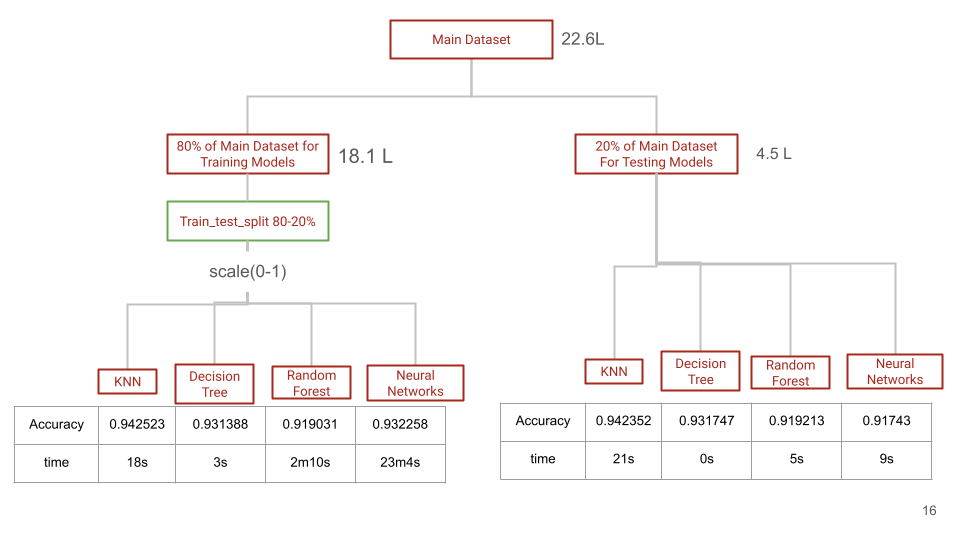
\includegraphics[width=1\linewidth]{Thesis Prashant//Images//Results/Classifier Results.png}
    \caption{Model Comparison on training and unknown data set}
    \label{fig:enter-label}
\end{figure}

%The results for different classification methods give accuracy during training period KNN $94.25\%$, Decision Tree  $93.13\%$, Random Forest $91.90\%$, and Neural Networks $93.22\%$  in time 18s, 3s, 2min, and 23min respectively. And while using the exported model on a completely unknown data set  KNN $94.23\%$, Decision Tree  $93.17\%$, Random Forest $91.92\%$, and Neural Networks $91.74\%$ in time 21s, ~0s, 5s, and 9s respectively.










% Disable the next few lines if you do not require an appendix
\appendix
\appendixpage
\addappheadtotoc
\chapter{Data collection of three simultaneous sensors}

The electrical resistance of the thin films was monitored in reaction to different volatile organic compounds (VOCs) at constant operating temperatures in order to conduct gas-sensing studies. Under dynamic flow conditions set by mass flow controllers with different capacities, the sample gases were infused. 
\begin{figure}
    \centering
    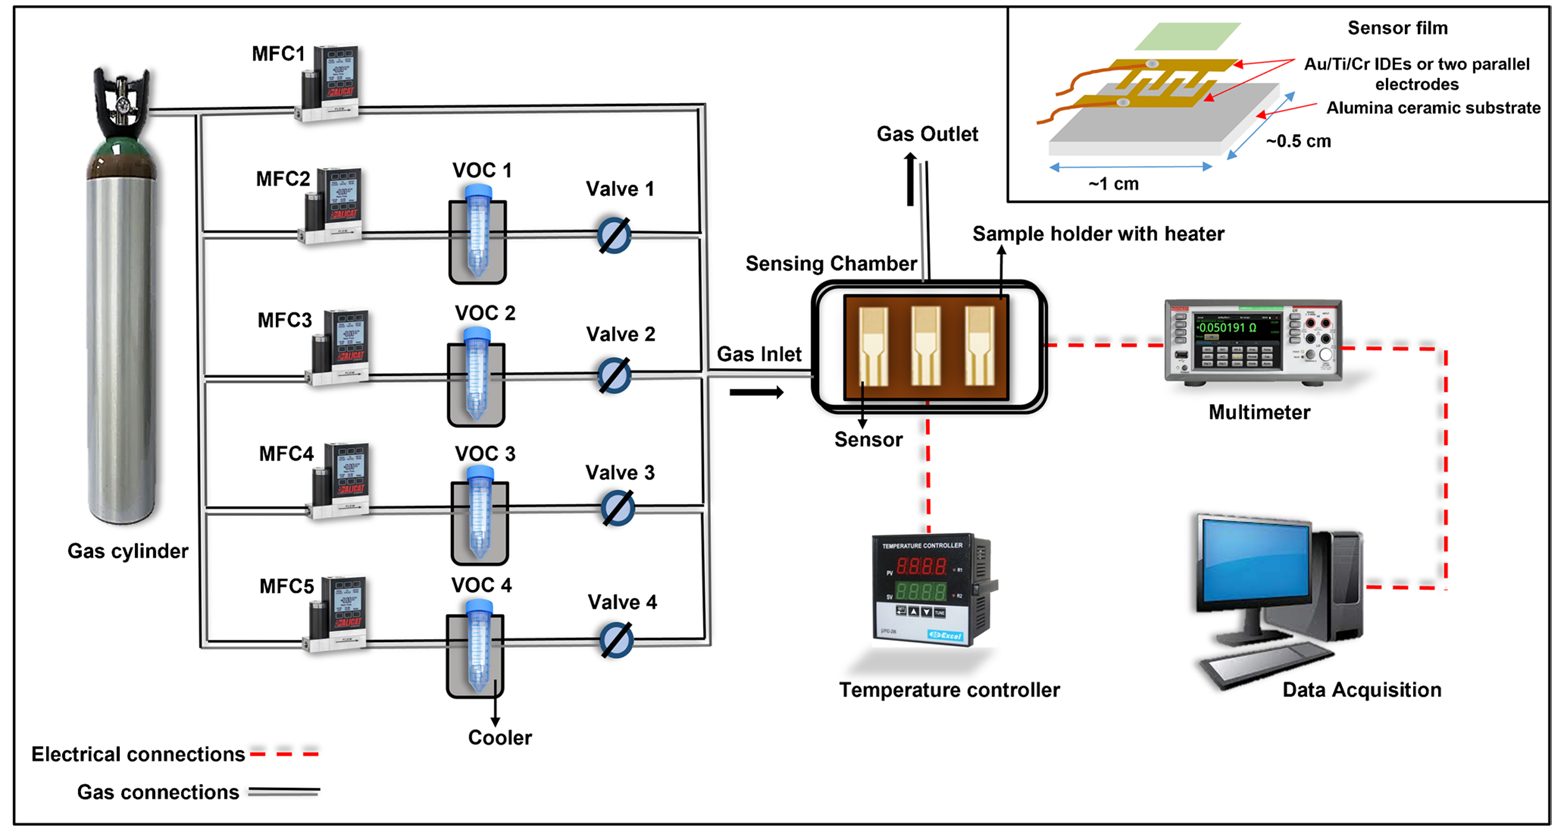
\includegraphics[width=1\linewidth]{Thesis Prashant//Images//Figures/gas sensing setup.png}
    \caption{ The schematic diagram of the gas sensing setup used for the experiment \cite{singh2024metal}}
    \label{fig:enter-label}
\end{figure}
The in-house gas sensing system employed in this study is shown in Figure 1. In order to assess the gas sensing characteristic in a detecting chamber, the films were placed on a sample holder that could achieve 400°C utilizing a heater underneath the sample holder (manufactured by Excel Instruments, India). The temperature of the sensor was determined using a sample holder with a type-K thermocouple installed. For measuring sensor resistance, an alumina substrate with interdigitated gold electrodes is used. The sensor resistance was measured using a Keithley 6517B electrometer connected to a workstation by providing two probes with a constant bias voltage of 10 V. With a tolerance of 1 fA, it is a high-resistance analyzer that could contribute meaningfully to  1015 ohms. To evaluate the sensor sensitivity to ethanol and other volatile organic compounds, the deposited films need to be exposed to the relevant vapours diluted in the air. \cite{singh2024metal}






\chapter{Building Thermal Expansion Measurement System
and its interfacing} 
\label{Appendix A}

\section{Building Thermal Expansion Measurement System
and its interfacing}
\subsection{The principle of measurement system}
The coefficient of linear Thermal expansion ($\alpha$) denotes the change in length of the given
material when heated. It is a material property and the same may be written as, $$\alpha = \frac{\frac{L_{f}-L_{0}}{L_{0}}}{T_{f}-T_{0}}$$
The quantity is of high significance for studying the thermal properties of materials for
fundamental as well as applied areas. A couple of methods have been reported for the measurement of TEC. Those can be broadly classified
as-
\begin{itemize}
    \item Interferometry - light interference based
    \item Diletometry
    \item Capacitance based
    \item LVDT-based
\end{itemize}
In the case of interferometric methods, the sample surface is shone with a monochromatic light beam, and the interference fringes are observed from the rays reflected on the surface. Although this method has high precision, it is applicable to only a limited range of $\alpha$ values and depends on the sample surface optical properties.\\
On the other hand, in dilatometric methods, the change in length of the material is measured by means of a linear translation rod/arm assembly that changes the signal on the capacitance bridge or an LVDT, respectively. We have developed a system based on this method using a Linear Variable Differential Transformer (LVDT) as a linear transducer.
\subsection{Instrumentation}
The entire system is home built and the schematic diagram of the system is shown in Fig 2.8. 
\begin{figure}
    \centering
    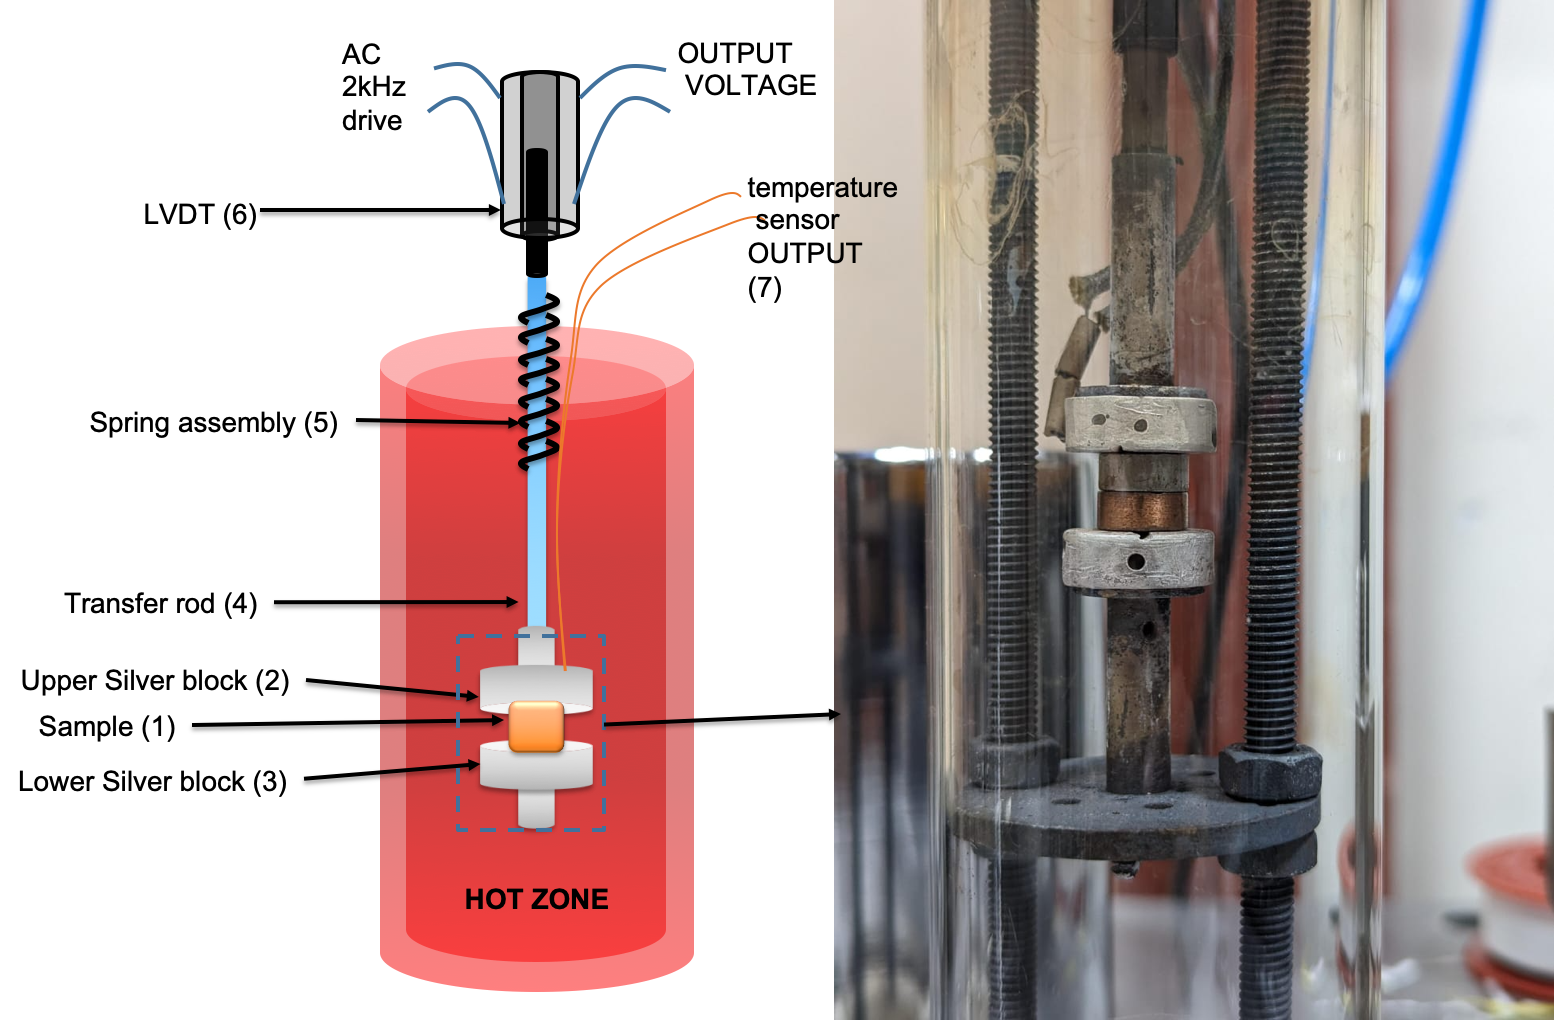
\includegraphics[width=1\linewidth]{Thesis Prashant//Images//media/image9.png}
    \caption{The schematic diagram of the home built Thermal expansion measurement system and its digital
photograph.}
    \label{fig:enter-label}
\end{figure}
The sample (1) to be measured is sandwiched between two silver metal blocks (2 and 3) for to hold in place, as well as silver helps in better temperature equilibration. The lower silver block is fixed while the upper silver block is mounted on a transfer rod/arm (4) which is made up of steel (not modified to Quartz). For this top silver block to always press against the sample, it is equipped with a spring assembly (5) that always pushes it against the sample. This ensures that
any change is sample length is directly translated to the other end of the rod where the transducer is place. As mentioned above, LVDT is used here as a transducer as shown in the figure.
The enlarged view of sample holder assembly is also shown in Fig 1. The entire sample
holder goes inside a vacuum chamber made of the quartz tube with suitable couplers and flanges.
The Quartz tube is inserted into the furnace (hot zone) to raise the sample temperature uniformly.
A k-type thermocouple is inserted in upper silver block to measure the sample temperature. The
electronic components are place away from the hot zone. If the sample is placed, it is expected to show a certain signal from the LVDT arm. If its temperature is raised and it expands the change is length of the sample caused the quartz rod to
push the core of LVDT further inside producing a change in signal.

\subsubsection{Design and working of LVDT}
An AC power source of 1.2 V at 2 kHz sine wave was used to power the LVDT, and a Keithley
2700 Multi-meter cum data acquisition system was used to read its analog outputs.
\begin{figure}
    \centering
    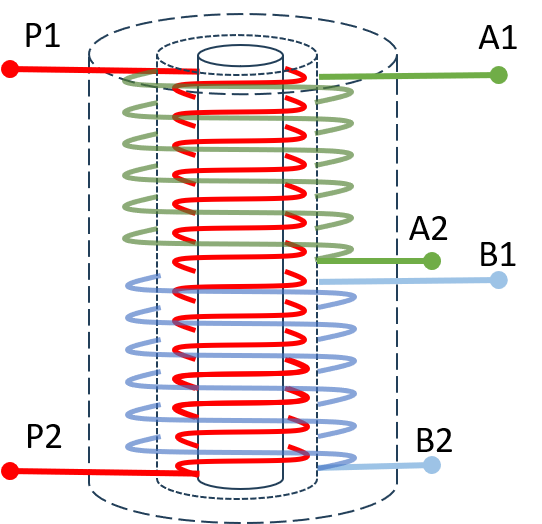
\includegraphics[width=0.5\linewidth]{Thesis Prashant//Images//media/image10.png}
    \caption{Circuit diagram of LVDT primary winding and Secondary winding.}
    \label{fig:enter-label}
\end{figure}
A hollow cylinder of insulating material serves as its main component. This insulating cylinder has one main winding P and two secondary winding A and B looped around its circumference. In the middle of the insulating cylinder lies the main winding P, and on either side of it are two secondary winding, A and B, coiled in complete opposition to one another as shown in Fig 2.9 In other words, A and B are moving in opposite directions. A magnetic or armature core is put within the insulating hollow cylinder and can move freely in both directions. Attaching the soft iron core to the object under study allows for the measurement of displacement. Nickel is commonly used in soft-core because of its great sensitivity. [9]
\begin{figure}
    \centering
    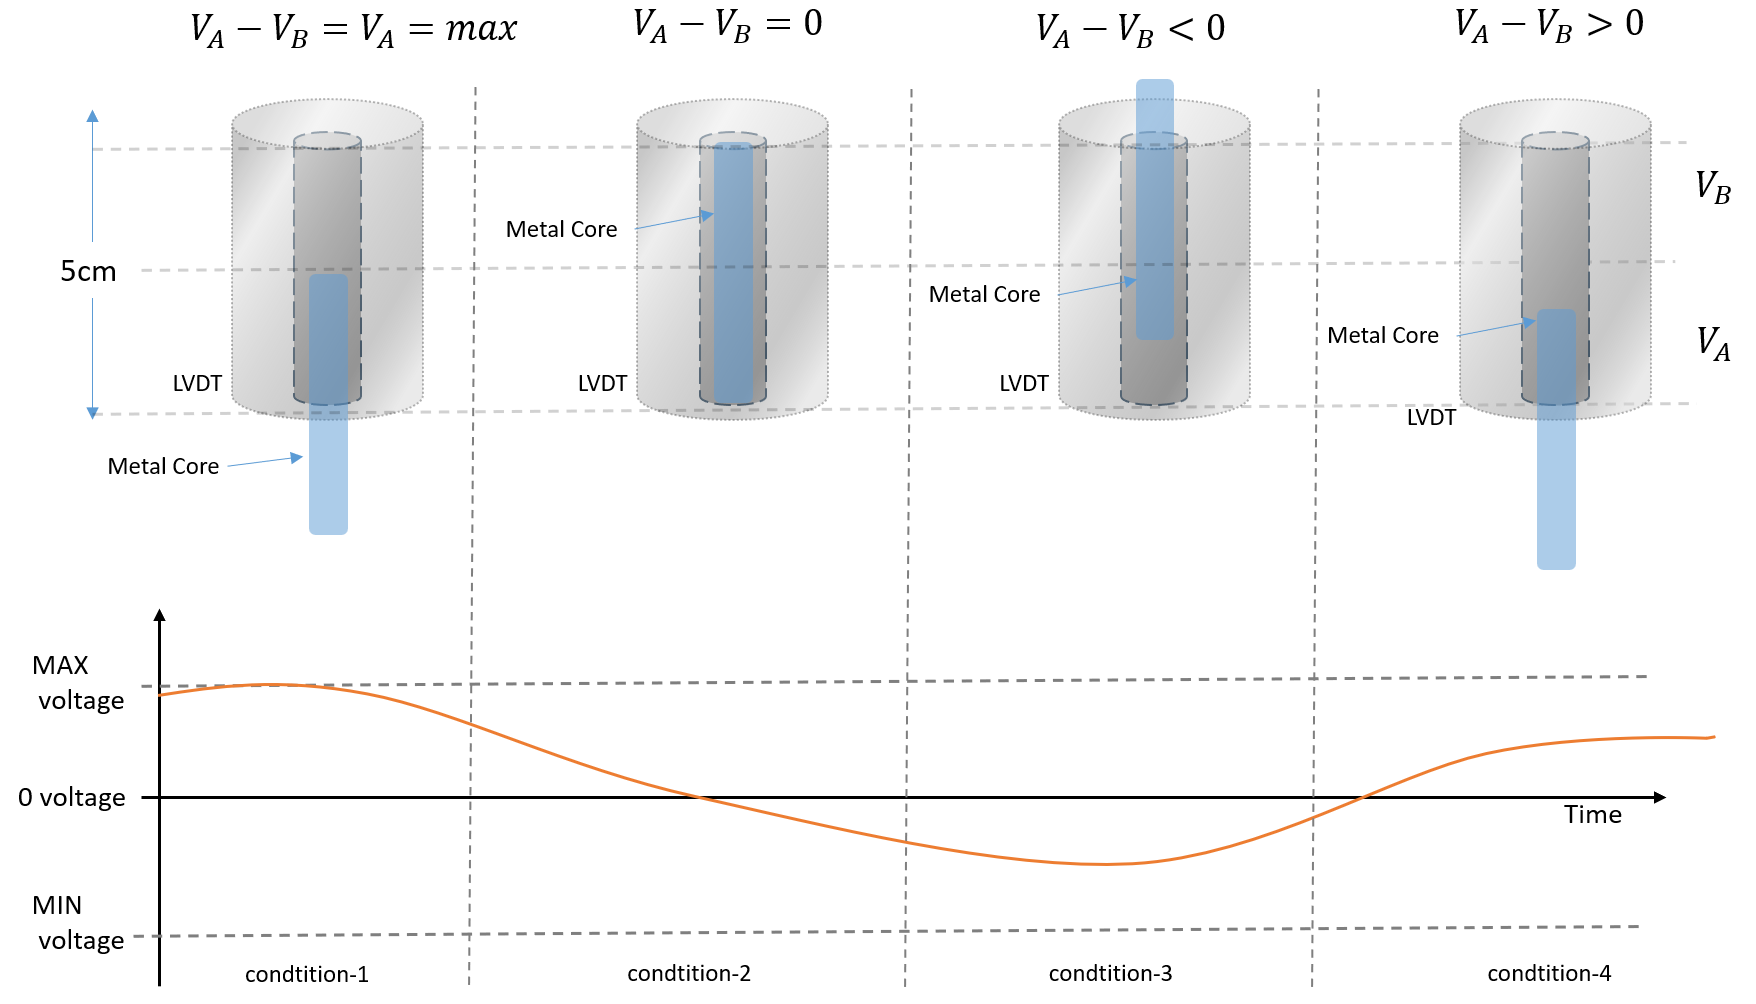
\includegraphics[width=0.8\linewidth]{Thesis Prashant//Images//media/image11.png}
    \caption{Different placements of metal core inside LVDT and corresponding voltage signal
being generated.}
    \label{fig:enter-label}
\end{figure}

From Faraday’s law of electromagnetic induction, an EMF is produced in the secondary winding. When the primary winding is supplied with an alternating current, a magnetic flux is generated that travels through both A and B. Primary winding flux is proportional to secondary winding conductor count. The primary coil is powered using an AC signal (here we used 2 kHz and 1.2 V). The magnetic induction into the secondary develops due to magnetic core placed in between (like a transformer). When the core of LVDT may slide to shifts to top, bottom or to the null position. There will be an increase or decrease in the output difference. In this case, the LVDT's output voltage is a linear function of core displacement up
to a certain point (5 mm from the LVDT's null position limit). This graph displays the variation in output voltage versus displacement. (See Fig 2.10 ).

Measuring TEC requires monitoring the output voltage of the LVDT that changes when the temperature of the sample under consideration varies. With increment in temperature, material expands and so the connected shaft to the metal core inside LVDT moves, which gives change in voltage proportional to the change in position of the metal core. Therefore, LVDTs can
be consider as length or position sensors that detect changes in length or position.

In order to measure the TEC a change in length of material with change of temperature is to be measured, and initial length of the sample should be known. With a good sensitive LVDT even a small expansion (sub mm) can also be measured accurately. Thus, the final system measurement should give the plot between change in length vs temperature. Change in length becomes change in Voltage by using LVDT’s sensitivity factor (typically given in mV/mm).

Let $V_{A}$ and $V_{B}$ be the voltages produced by the A and B coil, respectively. Since A and B are connected in opposite directions, they must be connected in series to create a single voltage with a phase difference of 180 degrees. Because of this, the secondary coil's output will be the difference between the two voltages produced by the device.
$$V = V_{A}-V_{B}$$
The secondary coil’s voltage output is linear for small displacements, as seen in Fig 12. There are no discrete steps in the voltage output, and the resolution is more a function of the testing apparatus than the transducer itself. No further intermediary amplifiers are required since the output voltage is large and easily measurable. The transducer can withstand significant vibration and stress because of its high sensitivity. Most importantly, the measuring system is insensitive to changes in temperature and suffers no loss due to friction. This attribute is necessary because of its proximity to a high-temperature furnace.

\subsection{Calibration and Measurement}
\textbf{Fig13}--- The preliminary measurements performed with the system are shown in Fig. The system
\begin{figure}
    \centering
    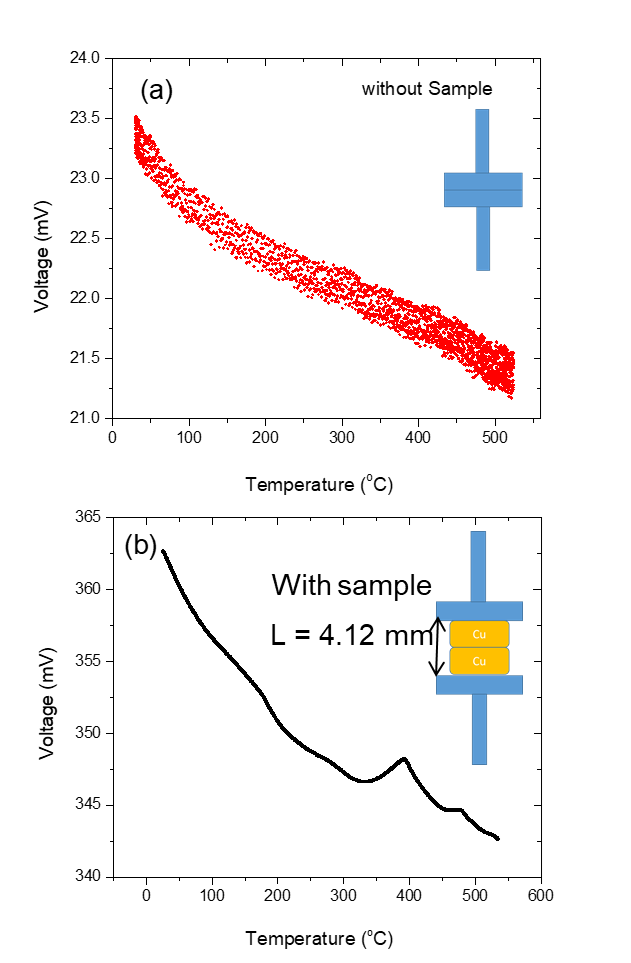
\includegraphics[width=0.5\linewidth]{Thesis Prashant//Images//media/image12.png}
    \caption{(a) Without and (b) With sample thermal expansion measurement data. Two Cu
samples in the stack (each with L = 4.12mm) were used as samples.}
    \label{fig:enter-label}
\end{figure}
background data was measured without any sample and shown in Fig (a). because of the
component used for sample holder there were non-zero background signal measured. Because
of its low value there is a significant noise in the background. Similarly, the data was also
measured by placing a sufficiently long Cu sample(s) between the two silver holders. This
yielded about one order of magnitude large change in the voltage. Cu is used here for
standardization for its known and high value of TEC. 
Nevertheless, there are several non-monotonous changes in the voltage that are not expected.

\begin{figure}
    \centering
    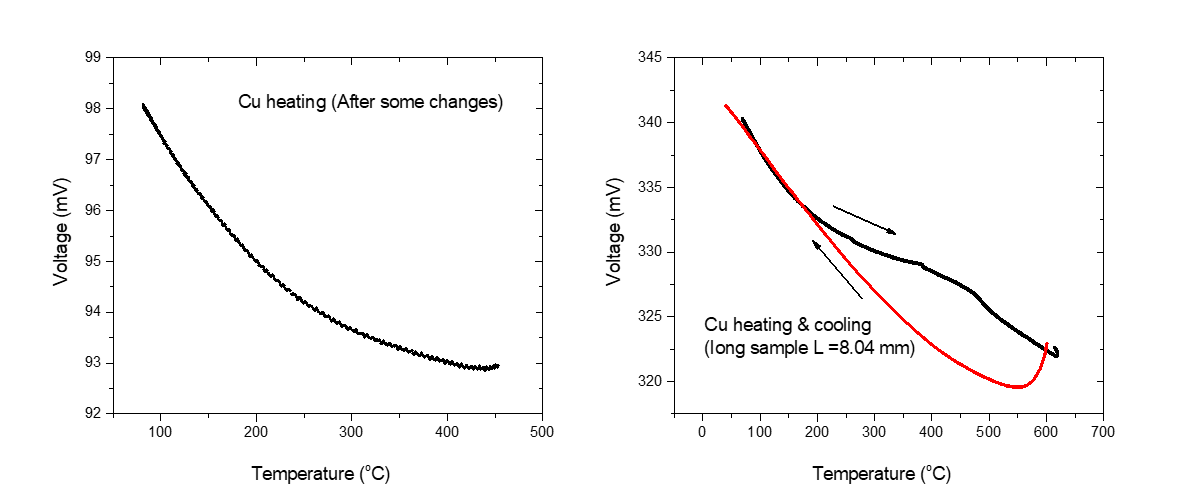
\includegraphics[width=0.8\linewidth]{Thesis Prashant//Images//media/image13.png}
    \caption{Measurements performed on the (a) same Cu sample, L= 4.12mm and (b) longer sample (8.04
mm length Cu sample)}
    \label{fig:enter-label}
\end{figure}
Further, optimization of the system needs dynamic measurements. Also, the
final data is to be represented as ΔL/L. Here, copper has very high thermal expansion coefficient. However, for insulating samples like ceramics etc. the TEC value is low and hence the is of the order of background. In that case, it will be challenging to analyze the result when signal to noise ratio is low.

\section{Thermal Expansion Temperature v/s Voltage}

\begin{figure}
    \centering
    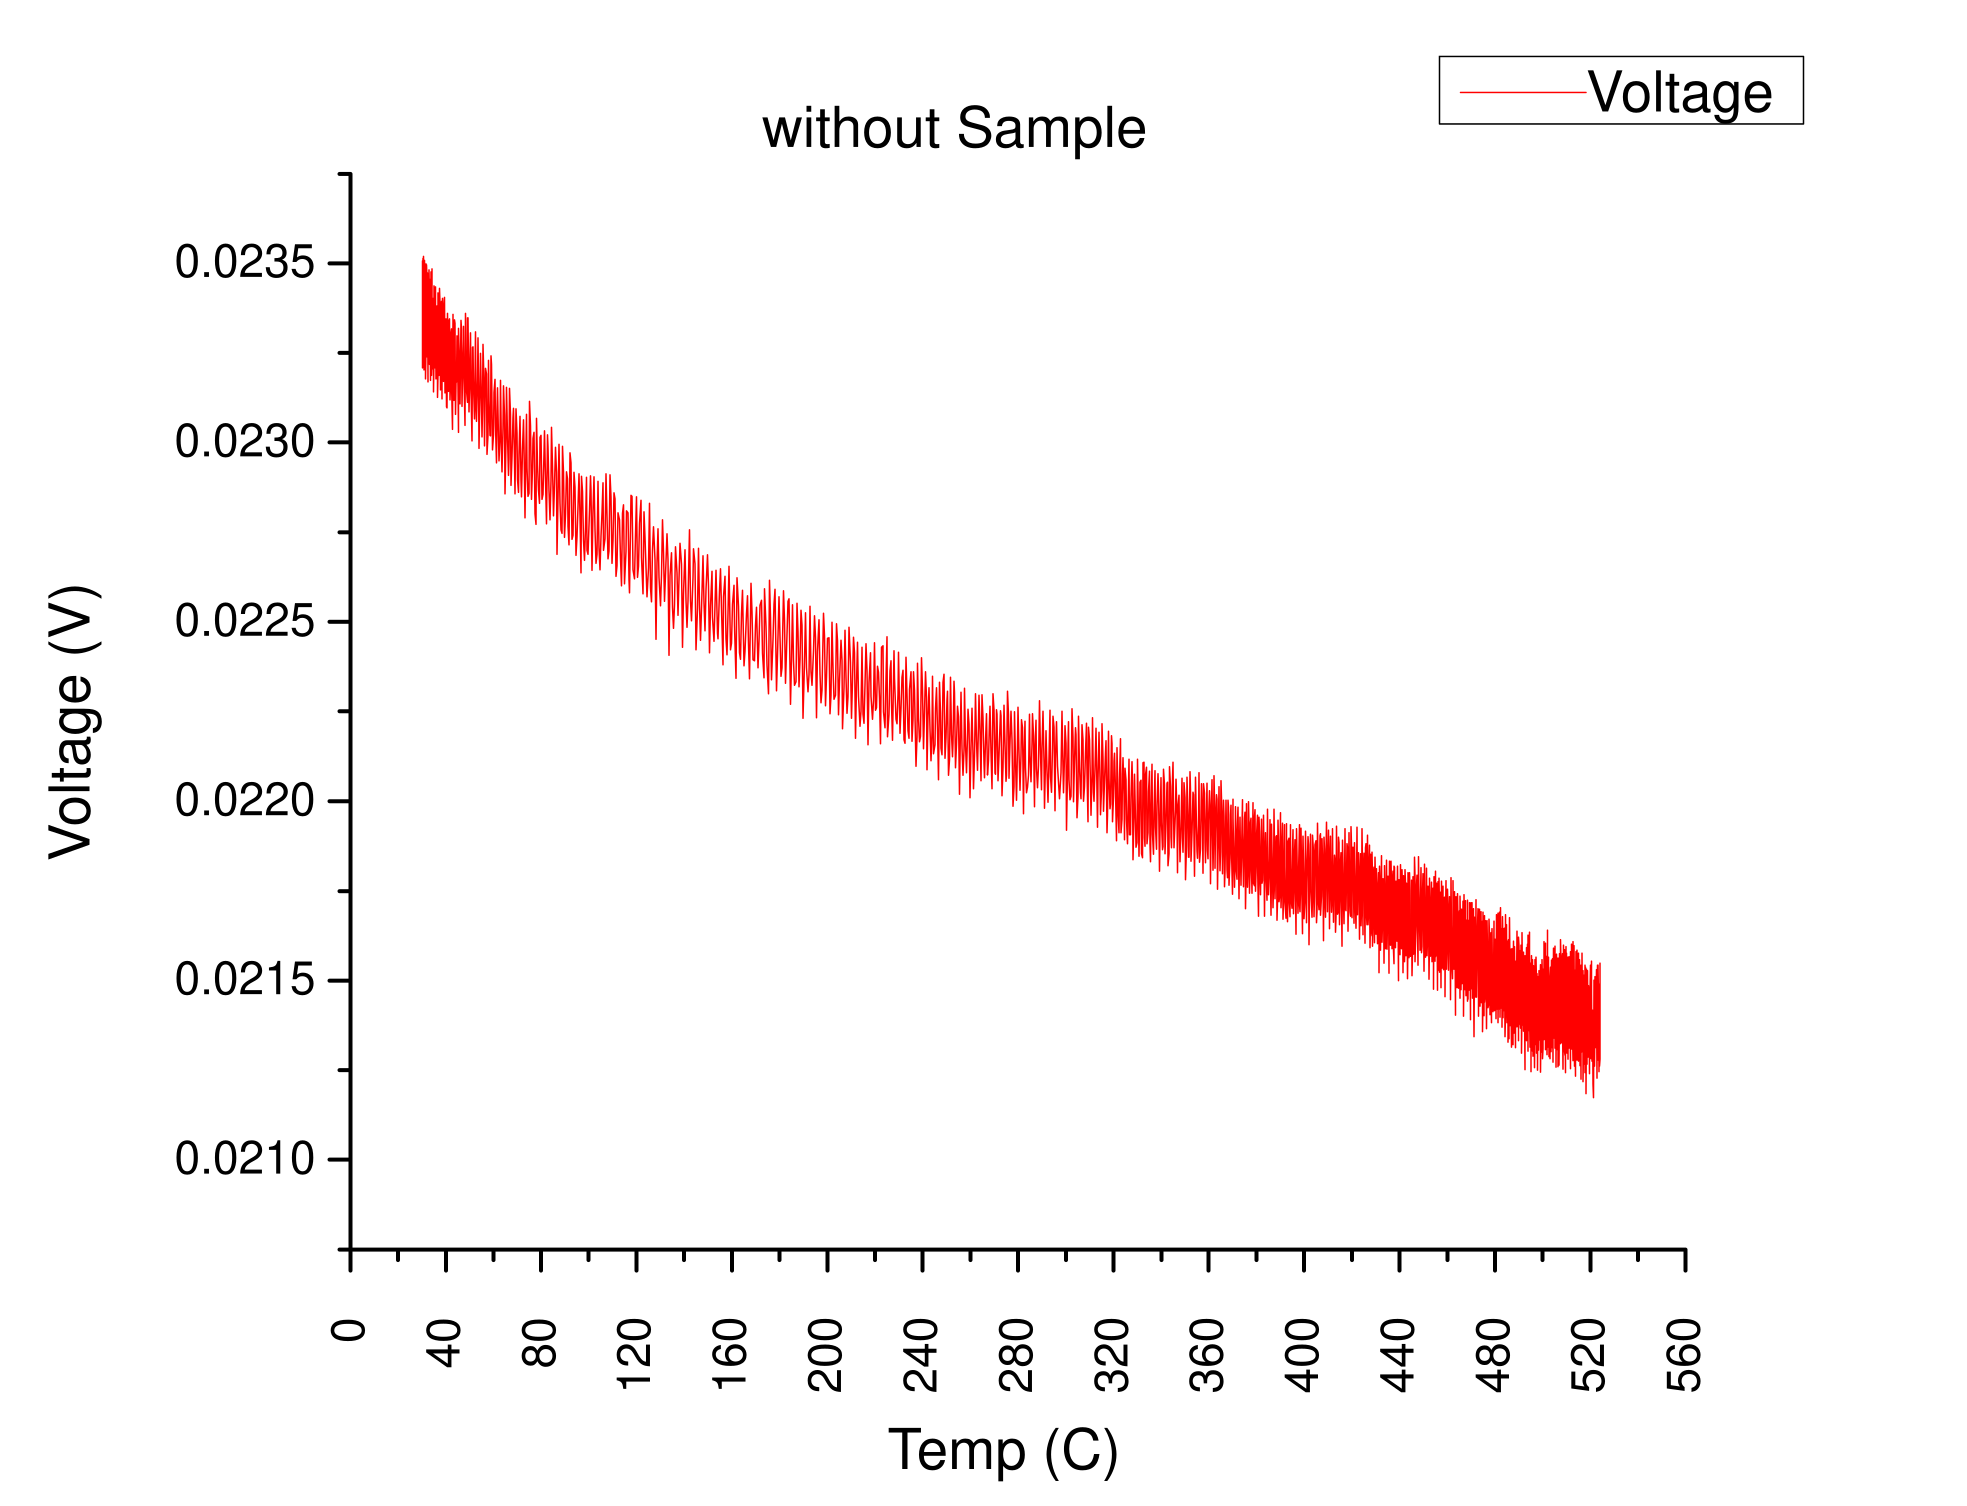
\includegraphics[width=0.6\linewidth]{Thesis Prashant//Images//media/image22.png}
    \caption{without sample thermal expansion measurement}
    \label{fig:enter-label}
\end{figure}



\nocite{*} % Without this, only cited materials are displayed in the bibliography.
\printbibliography[heading=bibintoc] % adds bibliography to ToC

\end{document}